\documentclass[aspectratio=169]{beamer}

\usepackage[T5]{fontenc}
\usepackage[utf8]{inputenc}
\usepackage{lmodern}

\usetheme{Madrid}

\usepackage{graphicx}
\usepackage{multicol}
\usepackage{amsmath,amssymb}

% Outline look: blue text, numbered, no balls
\setbeamertemplate{section in toc}{%
  \leavevmode\inserttocsectionnumber.~\inserttocsection\par}
\setbeamercolor{section in toc}{fg=blue}

\hypersetup{colorlinks=true, urlcolor=blue}

\newcommand{\backbtn}{%
  \hfill\hyperlink{outline}{\beamerbutton{Mục lục}}}


% Giảm khoảng cách trên/dưới công thức hiển thị để slide gọn hơn
\makeatletter
\def\tight@disp{\setlength\abovedisplayskip{4pt plus 2pt}%
  \setlength\belowdisplayskip{4pt plus 2pt}%
  \setlength\abovedisplayshortskip{2pt plus 1pt}%
  \setlength\belowdisplayshortskip{2pt plus 1pt}}
\g@addto@macro\normalsize{\tight@disp}
\g@addto@macro\small{\tight@disp}
\g@addto@macro\footnotesize{\tight@disp}
\g@addto@macro\scriptsize{\tight@disp}
\makeatother

\title[Xoắn]{Xoắn}
\author[© N. V. Sỹ]{Nguyễn Văn Sỹ}
\institute[TNUT]{%
  Bộ môn Hệ thống Công nghiệp \\
  Trường Đại học Kỹ thuật Công nghiệp \\
  \href{mailto:vansy@tnut.edu.vn}{vansy@tnut.edu.vn}}
\date[Cơ học vật liệu]{\large Cơ học vật liệu – Xoắn \\[0.5em] \footnotesize \copyright\ Nguyễn Văn Sỹ}

\begin{document}

\begin{frame}
  \titlepage
\end{frame}
%====================
\begin{frame}{Tài liệu tham khảo}
	\small
	F. P. Beer, E. R. Johnston, Jr., J. T. DeWolf, D. F. Mazurek,
	\emph{Mechanics of Materials}, 6th ed., McGraw-Hill, New York, 2012.
	
	\vspace{1em}
	\footnotesize\color{gray}
	Toàn bộ hình vẽ trong bài giảng được trích từ giáo trình trên, chỉ sử dụng
	cho mục đích giảng dạy nội bộ.
\end{frame}
% ===== OUTLINE SLIDE =====
\begin{frame}[t]{Nội dung}
  \hypertarget{outline}{}
  \tiny
  \begin{multicols}{2}
    \tableofcontents[hideallsubsections]
  \end{multicols}
\end{frame}

% ===== CONTENT SLIDES =====
\section{Tải trọng xoắn trên trục tròn}
\begin{frame}[t]{Tải trọng xoắn trên trục tròn}
  \begin{columns}[T]
    \column{0.52\textwidth}
      \small
      \begin{itemize}
        \setlength{\itemsep}{1em}
        \item Nghiên cứu ứng suất và biến dạng của trục tròn chịu tác
              dụng của các ngẫu lực xoắn, hay mô men xoắn.
        \item Tuabin tác dụng mô men xoắn $T$ lên trục.
        \item Trục truyền mô men xoắn đến máy phát.
        \item Máy phát tạo ra một mô men xoắn $T'$ bằng và ngược chiều.
      \end{itemize}
    \column{0.46\textwidth}
      \centering
      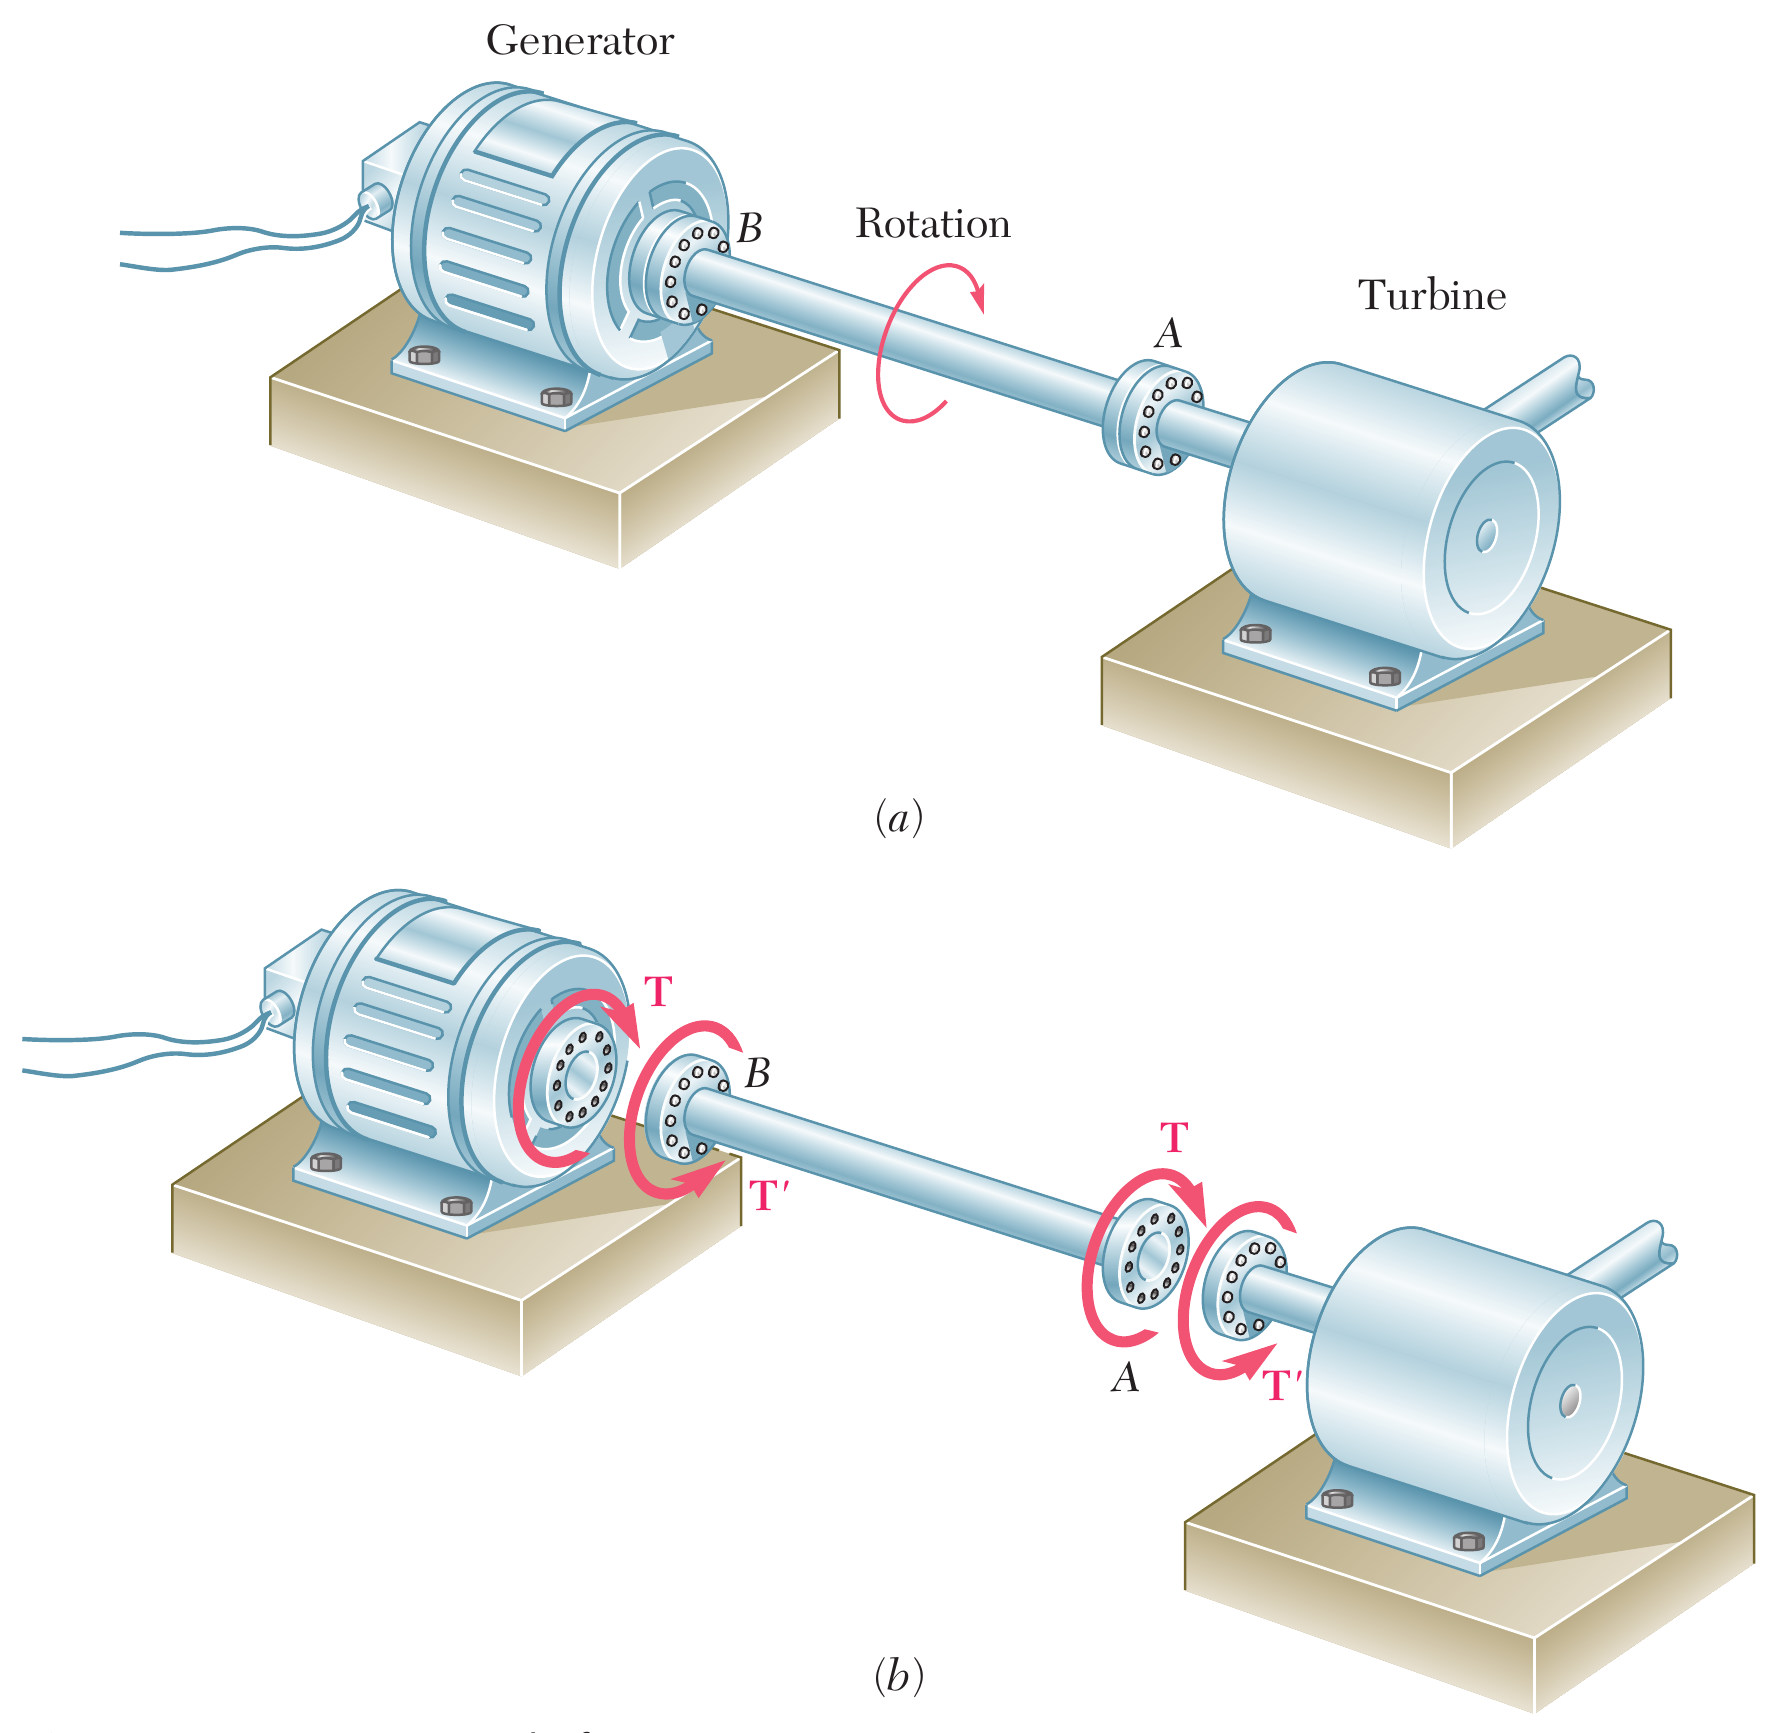
\includegraphics[width=\linewidth,height=5.5cm,keepaspectratio]{Chap_3/fig_3_2.png}
  \end{columns}
\end{frame}
% ===========
\section{Mô men xoắn tổng do nội ứng suất}
\begin{frame}[t]{Mô men xoắn tổng do nội ứng suất}
  \begin{columns}[T]
    \column{0.58\textwidth}
      \small
      \begin{itemize}
        \setlength{\itemsep}{0.6em}
        \item Tổng hợp của các ứng suất tiếp bên trong là một mô men xoắn
              nội lực, bằng và ngược chiều với mô men xoắn tác dụng:
        \[
          T = \int \rho\,dF = \int \rho(\tau\,dA)
        \]
        \item Mặc dù đã biết mô men tổng do ứng suất tiếp gây ra, nhưng
              phân bố của ứng suất thì chưa biết.
        \item Phân bố ứng suất tiếp là bài toán siêu tĩnh -- cần phải xét
              đến biến dạng của trục.
        \item Khác với ứng suất pháp do lực dọc trục, phân bố ứng suất
              tiếp do tải trọng xoắn không thể giả thiết là đều.
      \end{itemize}
    \column{0.40\textwidth}
      \centering
      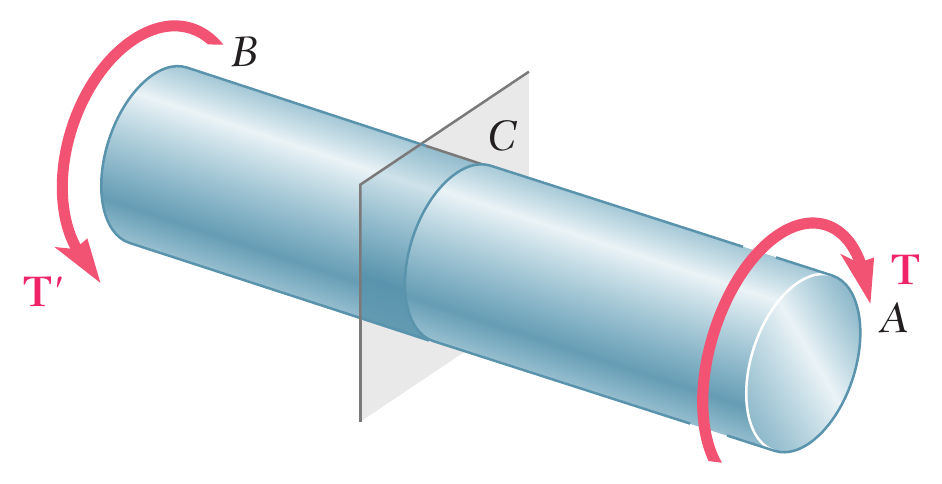
\includegraphics[width=\linewidth,height=2.9cm,keepaspectratio]{Chap_3/fig_3_3.png}\\[2pt]
      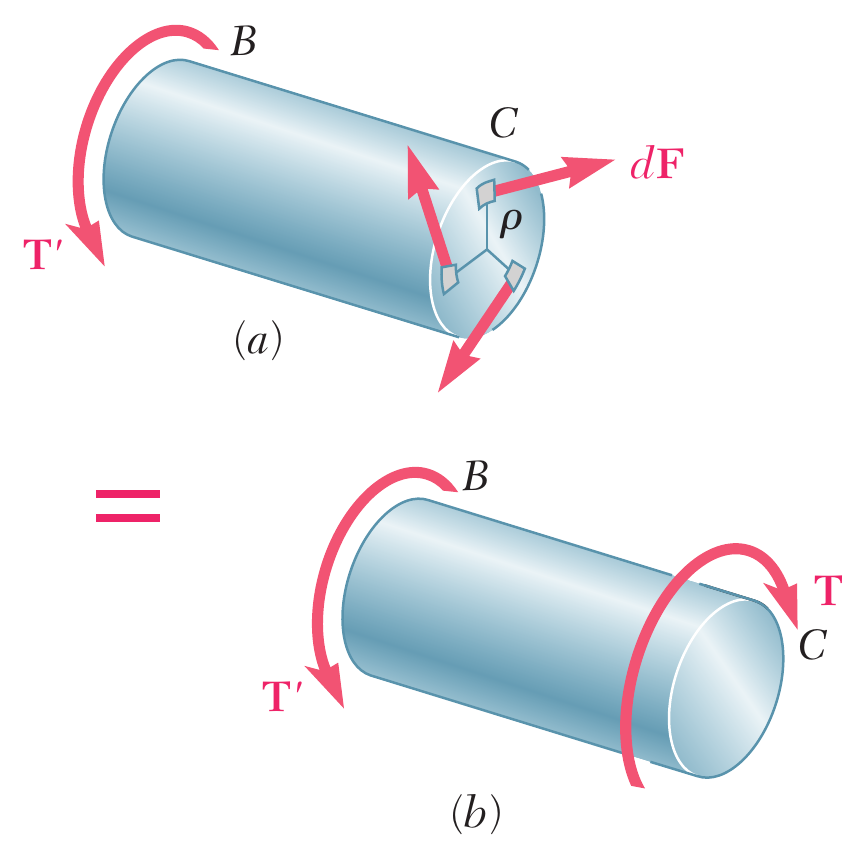
\includegraphics[width=\linewidth,height=2.9cm,keepaspectratio]{Chap_3/fig_3_4.png}
  \end{columns}
\end{frame}
% ===========
\section{Các thành phần ứng suất tiếp dọc trục}
\begin{frame}[t]{Các thành phần ứng suất tiếp dọc trục}
  \begin{columns}[T]
    \column{0.58\textwidth}
      \small
      \begin{itemize}
        \setlength{\itemsep}{0.7em}
        \item Mô men xoắn tác dụng lên trục gây ra ứng suất tiếp trên các
              mặt vuông góc với trục.
        \item Điều kiện cân bằng đòi hỏi phải tồn tại các ứng suất bằng
              như vậy trên các mặt của hai mặt phẳng chứa trục của trục.
        \item Sự tồn tại của các thành phần ứng suất tiếp dọc trục được
              minh họa bằng cách xét một trục ghép từ các thanh dọc.
        \item Các thanh trượt tương đối với nhau khi đặt các mô men xoắn
              bằng và ngược chiều ở hai đầu trục.
      \end{itemize}
    \column{0.40\textwidth}
      \centering
      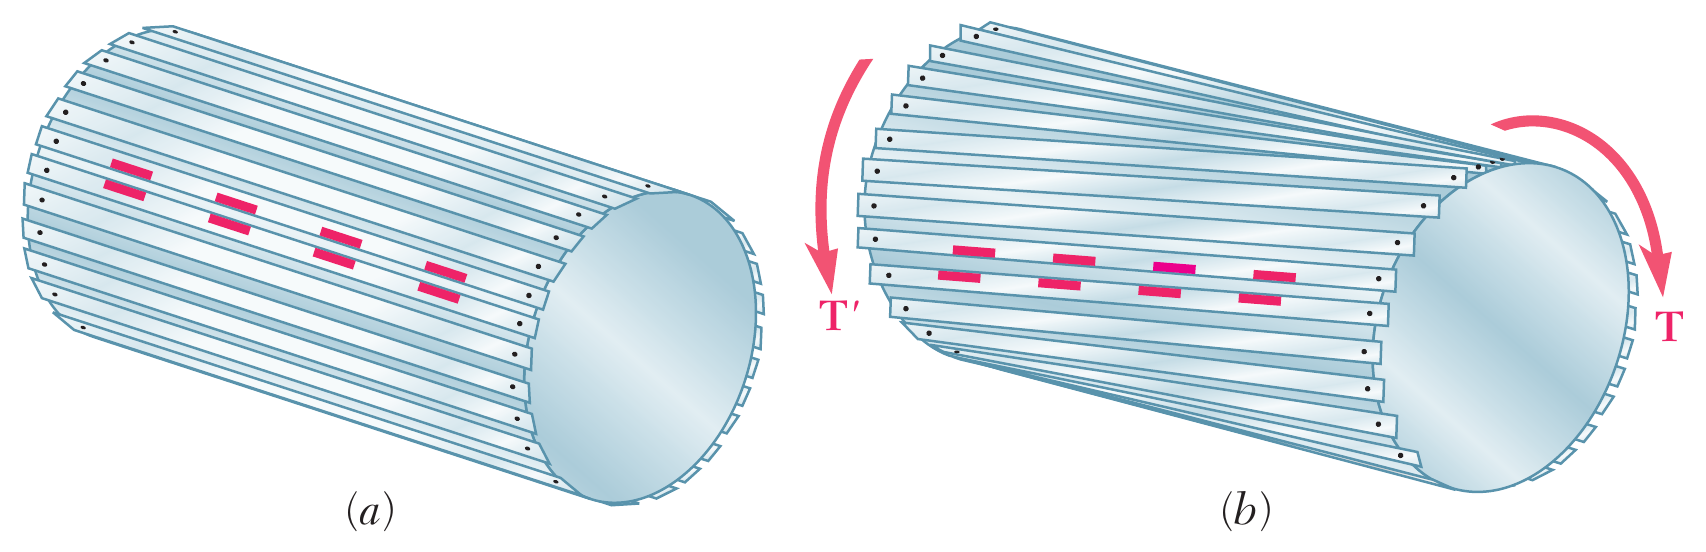
\includegraphics[width=\linewidth,height=5.5cm,keepaspectratio]{Chap_3/fig_3_6.png}
  \end{columns}
\end{frame}
% ===========
\section{Biến dạng của trục}
\begin{frame}[t]{Biến dạng của trục}
  \begin{columns}[T]
    \column{0.58\textwidth}
      \small
      \begin{itemize}
        \setlength{\itemsep}{0.6em}
        \item Từ quan sát, góc xoắn của trục tỉ lệ với mô men xoắn tác
              dụng và với chiều dài trục:
        \[
          \phi \propto T \qquad \phi \propto L
        \]
        \item Khi chịu xoắn, mọi mặt cắt ngang của trục tròn vẫn phẳng
              và không bị vênh.
        \item Mặt cắt ngang của trục tròn rỗng và đặc vẫn phẳng và không
              vênh vì trục tròn có tính đối xứng trục.
        \item Mặt cắt ngang của trục không tròn (không đối xứng trục) bị
              vênh khi chịu xoắn.
      \end{itemize}
    \column{0.40\textwidth}
      \centering
      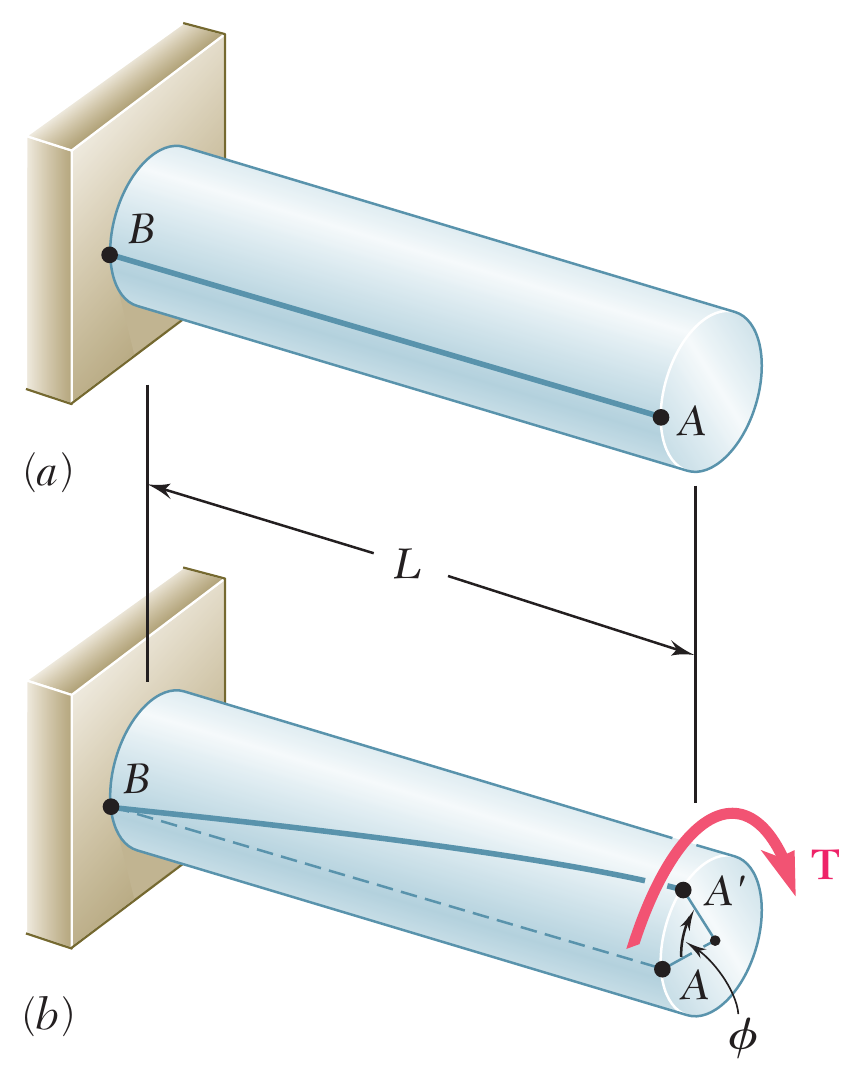
\includegraphics[width=\linewidth,height=2.9cm,keepaspectratio]{Chap_3/fig_3_7.png}\\[2pt]
      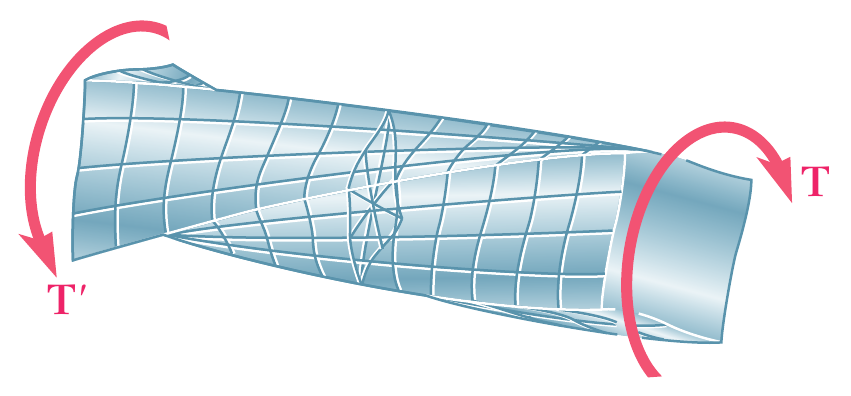
\includegraphics[width=\linewidth,height=2.9cm,keepaspectratio]{Chap_3/fig_3_42.png}
  \end{columns}
\end{frame}
% ===========
\section{Biến dạng trượt}
\begin{frame}[t]{Biến dạng trượt}
  \begin{columns}[T]
    \column{0.58\textwidth}
      \small
      \begin{itemize}
        \setlength{\itemsep}{0.7em}
        \item Xét một đoạn bên trong của trục. Khi đặt tải trọng xoắn,
              một phân tố trên mặt trụ bên trong biến dạng thành hình
              thoi.
        \item Vì hai đầu phân tố vẫn phẳng, biến dạng trượt bằng góc
              xoay tương đối:
        \[
          L\gamma = \rho\phi \quad\text{hay}\quad \gamma = \frac{\rho\phi}{L}
        \]
        \item Suy ra biến dạng trượt tỉ lệ với góc xoắn và bán kính:
        \[
          \gamma_{\max} = \frac{c\phi}{L}
          \quad\text{và}\quad
          \gamma = \frac{\rho}{c}\gamma_{\max}
        \]
      \end{itemize}
    \column{0.40\textwidth}
      \centering
      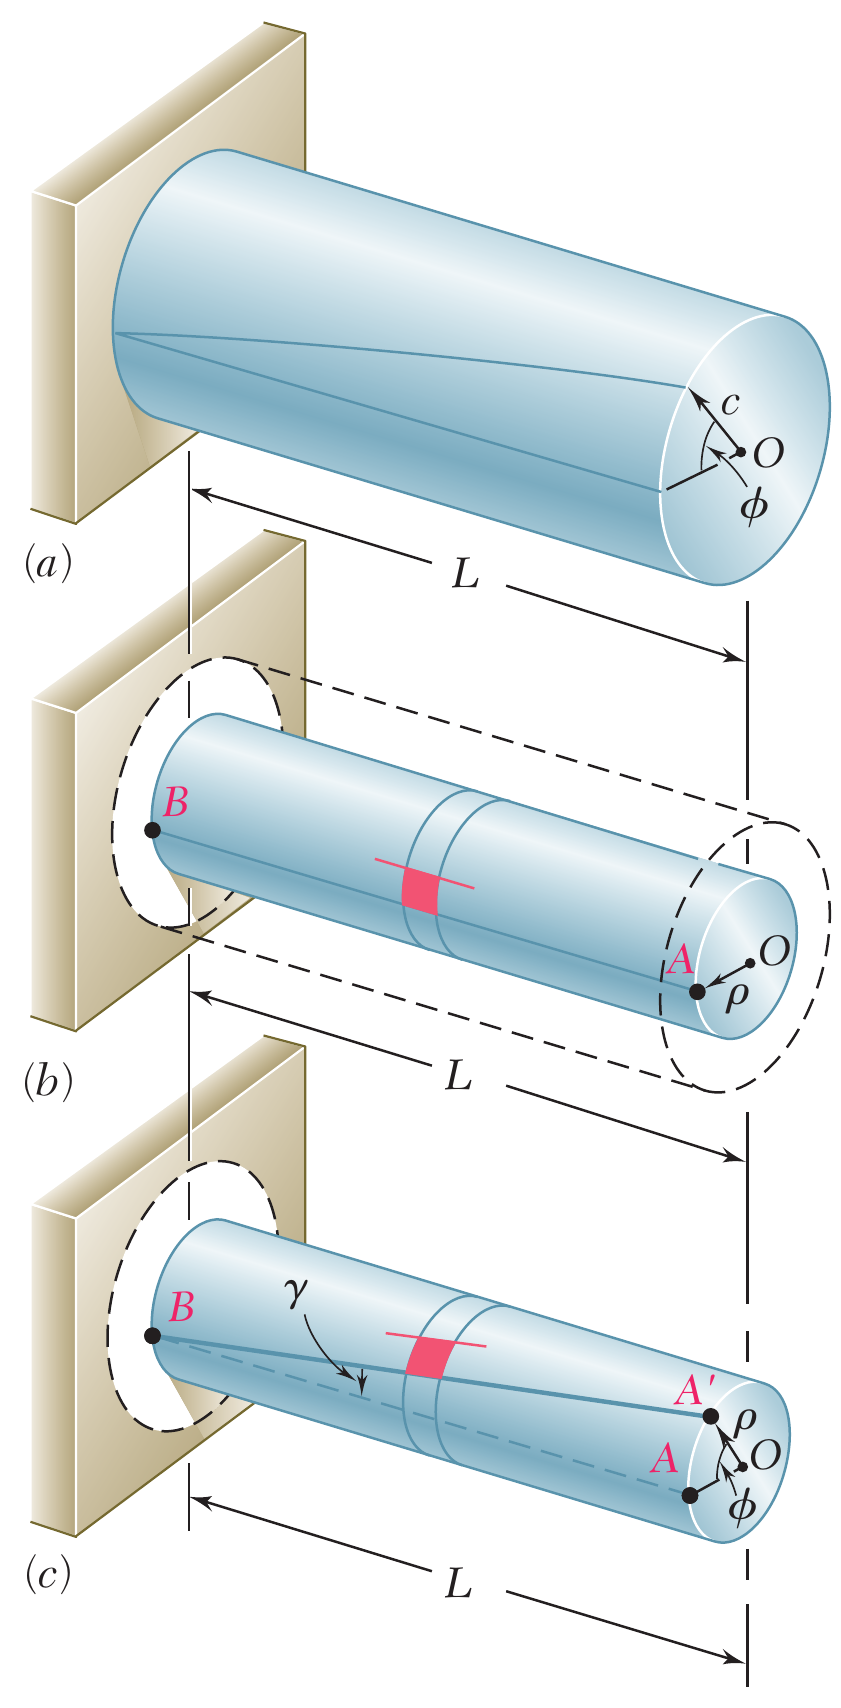
\includegraphics[width=\linewidth,height=5.5cm,keepaspectratio]{Chap_3/fig_3_13.png}
  \end{columns}
\end{frame}
% ===========
\section{Ứng suất trong miền đàn hồi}
\begin{frame}[t]{Ứng suất trong miền đàn hồi}
  \begin{columns}[T]
    \column{0.60\textwidth}
      \footnotesize
      \begin{itemize}
        \setlength{\itemsep}{0.4em}
        \item Nhân phương trình trước với mô đun trượt:
        \[
          G\gamma = \frac{\rho}{c}G\gamma_{\max}
        \]
        Theo định luật Hooke, $\tau = G\gamma$, nên
        \[
          \tau = \frac{\rho}{c}\tau_{\max}
        \]
        Ứng suất tiếp thay đổi tuyến tính theo bán kính trên mặt cắt.
        \item Nhắc lại: tổng mô men của phân bố nội ứng suất bằng mô men
              xoắn của trục tại mặt cắt:
        \[
          T = \int \rho\tau\,dA = \frac{\tau_{\max}}{c}\int\rho^2\,dA
            = \frac{\tau_{\max}}{c}J
        \]
        \item Các kết quả này được gọi là công thức xoắn đàn hồi:
        \[
          \tau_{\max} = \frac{Tc}{J} \quad\text{và}\quad
          \tau = \frac{T\rho}{J}
        \]
      \end{itemize}
    \column{0.38\textwidth}
      \centering
      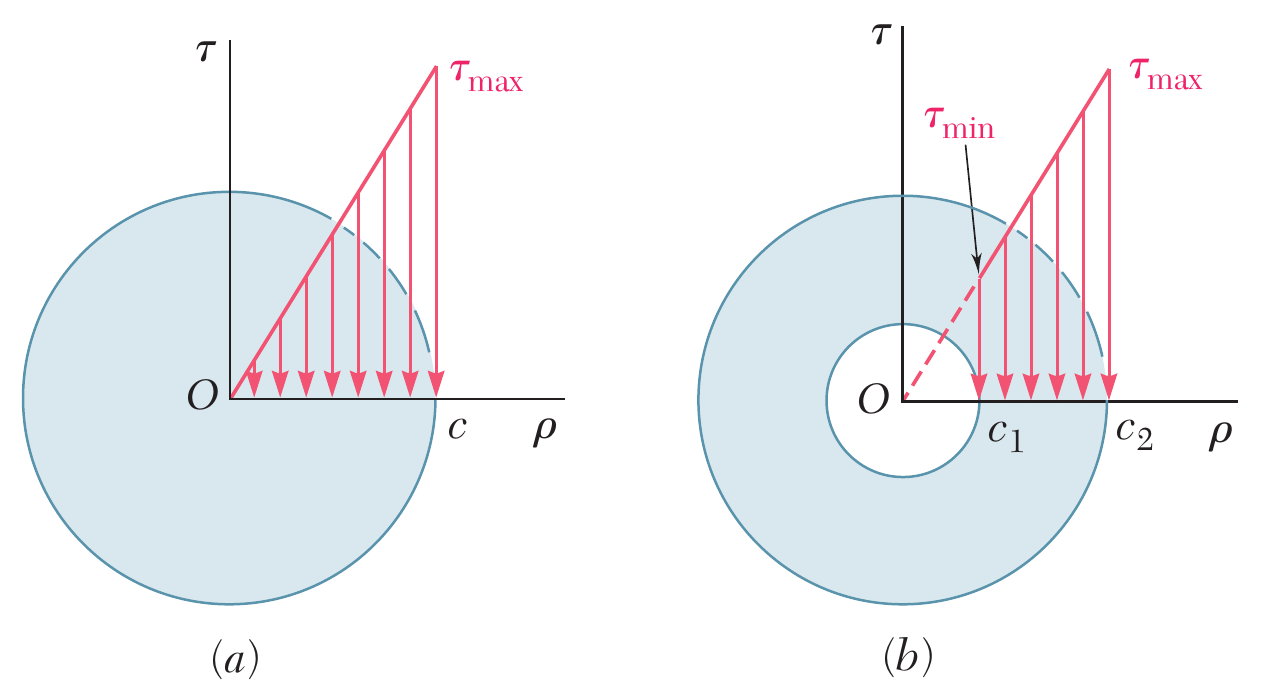
\includegraphics[width=\linewidth,height=2.6cm,keepaspectratio]{Chap_3/fig_3_14.png}\\
      \scriptsize $J = \tfrac{1}{2}\pi c^4$\\[2pt]
      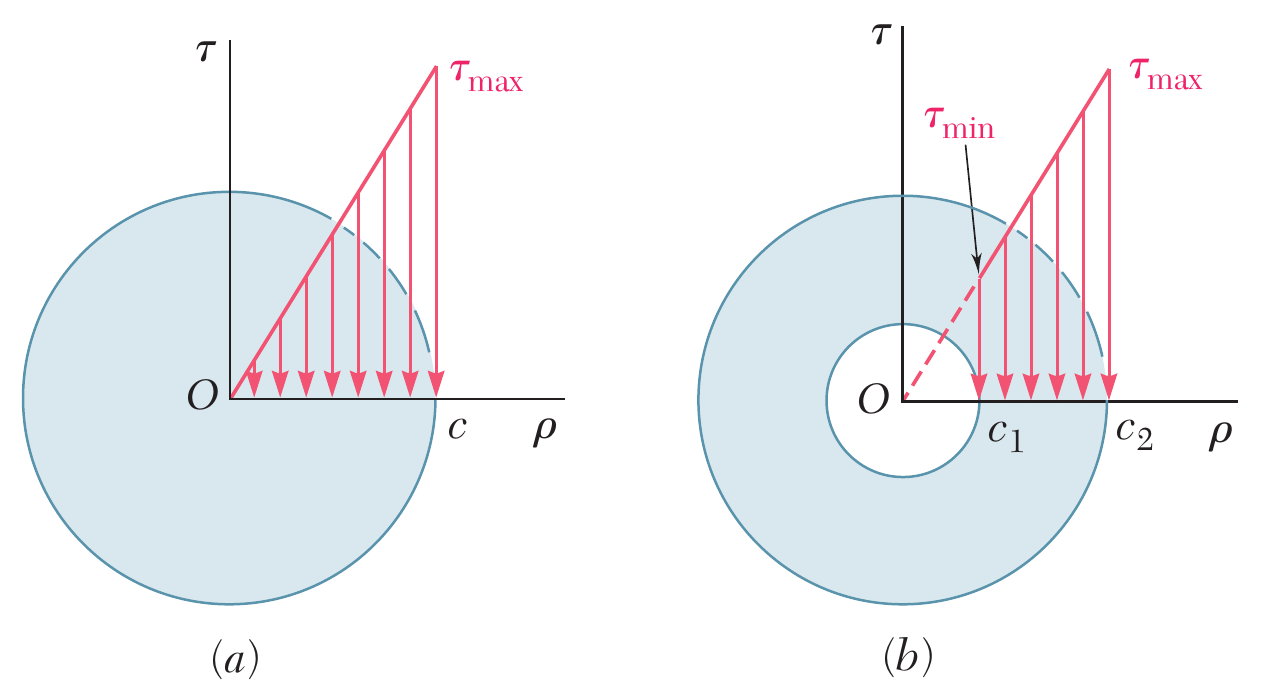
\includegraphics[width=\linewidth,height=2.6cm,keepaspectratio]{Chap_3/fig_3_14.png}\\
      \scriptsize $J = \tfrac{1}{2}\pi\left(c_2^4 - c_1^4\right)$
  \end{columns}
\end{frame}
% ===========
\section{Ứng suất pháp}
\begin{frame}[t]{Ứng suất pháp}
  \begin{columns}[T]
    \column{0.36\textwidth}
      \centering
      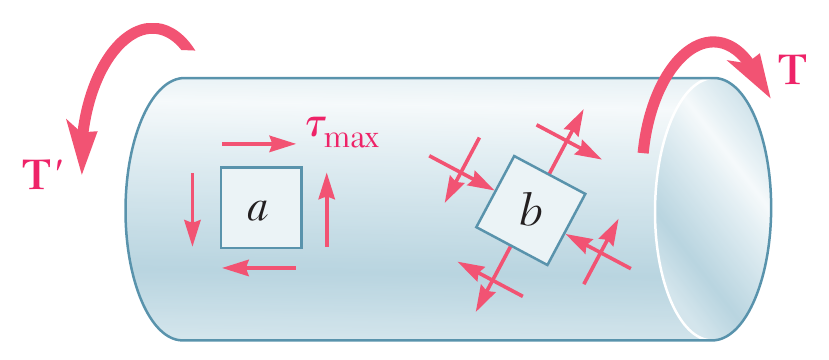
\includegraphics[width=\linewidth,height=1.9cm,keepaspectratio]{Chap_3/fig_3_17.png}\\[2pt]
      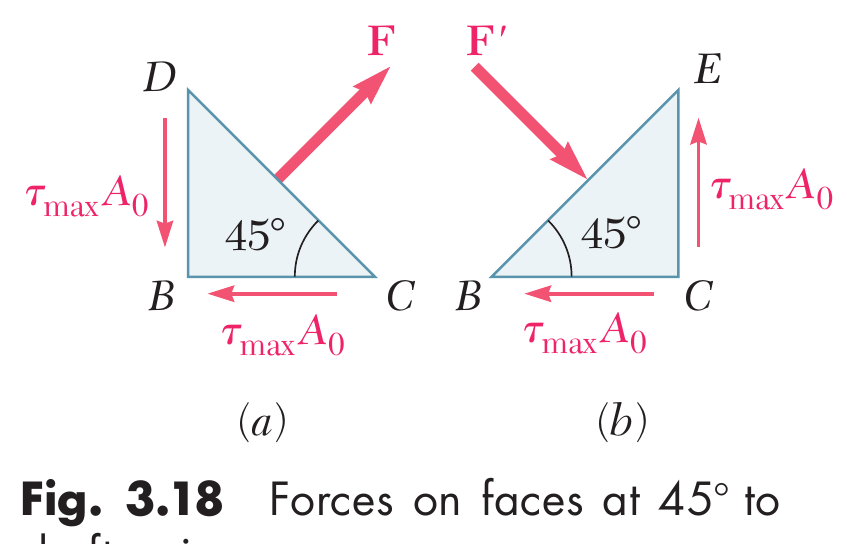
\includegraphics[width=\linewidth,height=1.9cm,keepaspectratio]{Chap_3/fig_3_18.png}\\[2pt]
      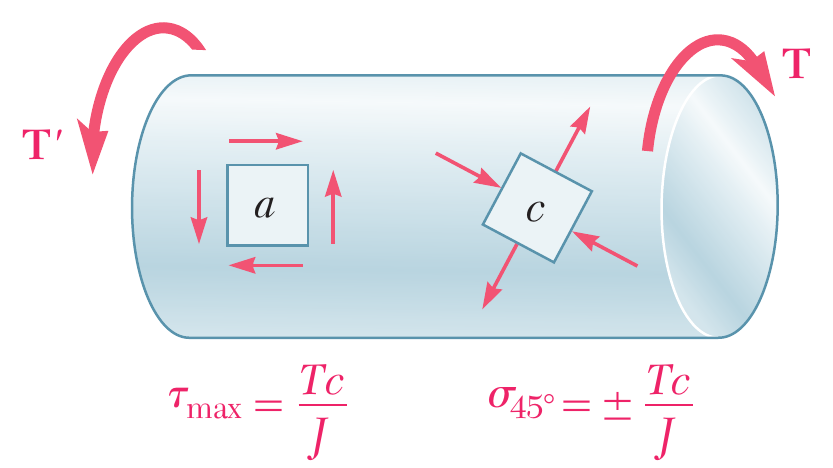
\includegraphics[width=\linewidth,height=1.9cm,keepaspectratio]{Chap_3/fig_3_19.png}
    \column{0.62\textwidth}
      \small
      \begin{itemize}
        \setlength{\itemsep}{0.5em}
        \item Các phân tố có mặt song song và vuông góc với trục của trục
              chỉ chịu ứng suất tiếp. Với các hướng khác có thể có ứng suất
              pháp, ứng suất tiếp hoặc tổ hợp của cả hai.
        \item Xét một phân tố nghiêng $45^\circ$ so với trục:
        \[
          F = 2(\tau_{\max}A_0)\cos 45^\circ = \tau_{\max}A_0\sqrt{2}
        \]
        \[
          \sigma_{45^\circ} = \frac{F}{A} = \frac{\tau_{\max}A_0\sqrt{2}}{A_0\sqrt{2}}
            = \tau_{\max}
        \]
        \item Phân tố $a$ ở trạng thái trượt thuần túy.
        \item Phân tố $c$ chịu ứng suất kéo trên hai mặt và ứng suất nén
              trên hai mặt còn lại.
        \item Lưu ý rằng mọi ứng suất của phân tố $a$ và $c$ đều có cùng
              độ lớn.
      \end{itemize}
  \end{columns}
\end{frame}
% ===========
\section{Các dạng phá hủy do xoắn}
\begin{frame}[t]{Các dạng phá hủy do xoắn}
  \begin{columns}[T]
    \column{0.58\textwidth}
      \small
      \begin{itemize}
        \setlength{\itemsep}{0.8em}
        \item Vật liệu dẻo thường bị phá hủy do cắt. Vật liệu giòn chịu
              kéo kém hơn chịu cắt.
        \item Khi chịu xoắn, mẫu vật liệu dẻo bị gãy theo mặt phẳng có
              ứng suất tiếp lớn nhất, tức là mặt phẳng vuông góc với trục.
        \item Khi chịu xoắn, mẫu vật liệu giòn bị gãy theo các mặt vuông
              góc với phương có ứng suất kéo lớn nhất, tức là theo các mặt
              nghiêng $45^\circ$ so với trục.
      \end{itemize}
    \column{0.40\textwidth}
      \centering
      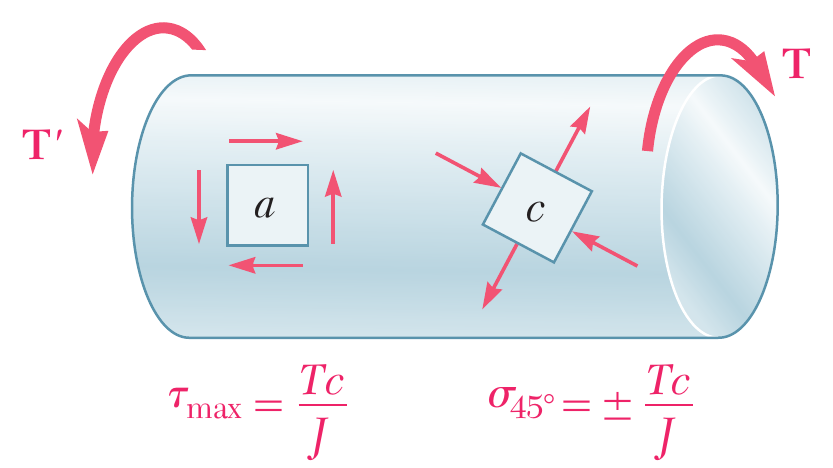
\includegraphics[width=\linewidth,height=1.9cm,keepaspectratio]{Chap_3/fig_3_19.png}\\[2pt]
      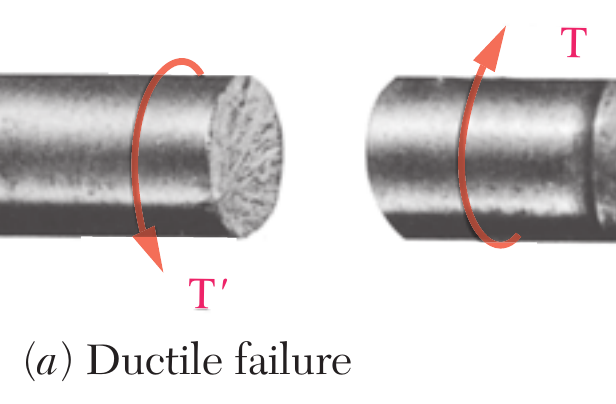
\includegraphics[width=\linewidth,height=1.9cm,keepaspectratio]{Chap_3/photo_3_2a.png}\\[2pt]
      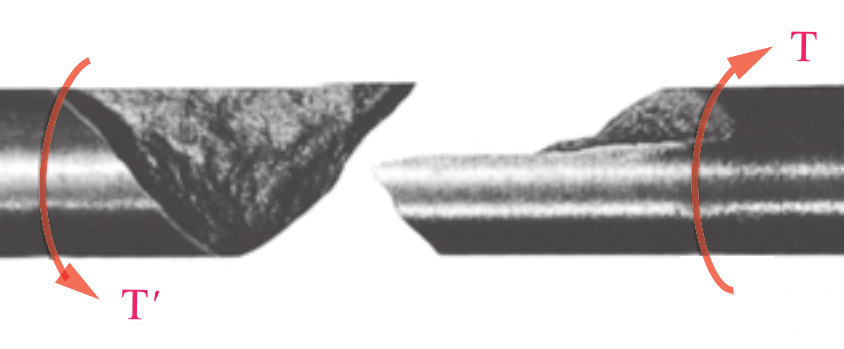
\includegraphics[width=\linewidth,height=1.9cm,keepaspectratio]{Chap_3/photo_3_2b.png}
  \end{columns}
\end{frame}
% ===========
\section{Bài mẫu 3.1}
\begin{frame}[t]{Bài mẫu 3.1}
  \begin{columns}[T]
    \column{0.40\textwidth}
      \centering
      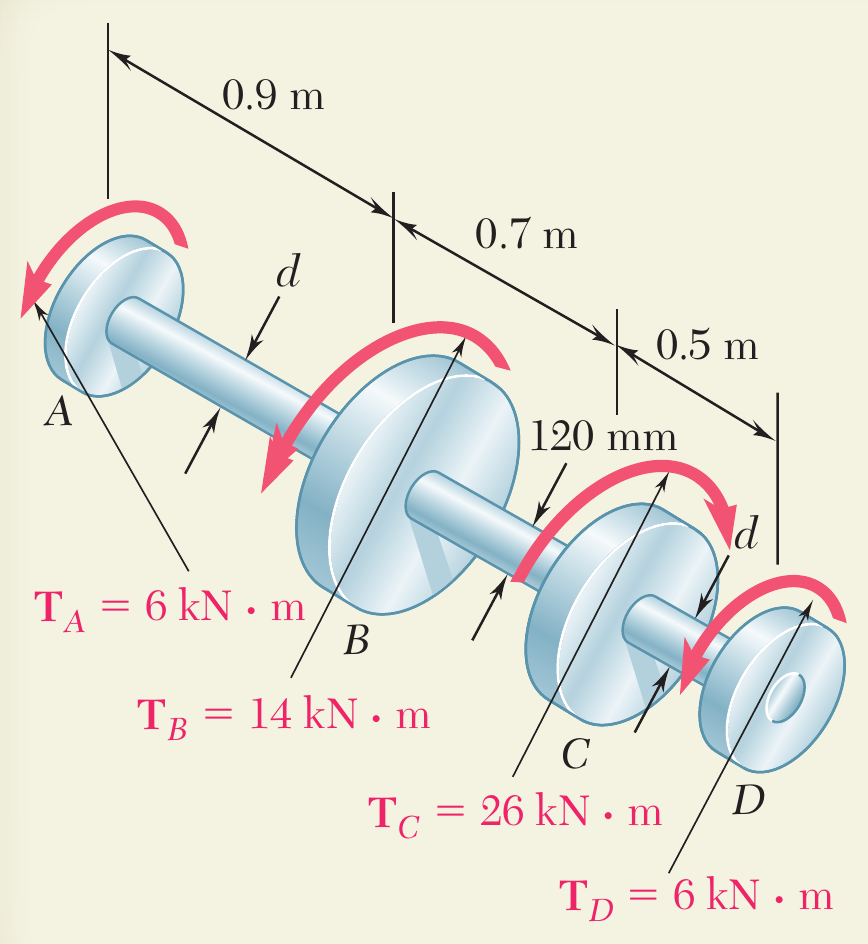
\includegraphics[width=\linewidth,height=5.5cm,keepaspectratio]{Chap_3/sp_3_1_a.png}
    \column{0.58\textwidth}
      \footnotesize
      Trục $BC$ rỗng có đường kính trong và ngoài lần lượt là 90 mm và
      120 mm. Các trục $AB$ và $CD$ đặc, đường kính $d$. Với tải trọng
      như hình vẽ, xác định (a) ứng suất tiếp nhỏ nhất và lớn nhất trong
      trục $BC$, (b) đường kính $d$ cần thiết của các trục $AB$ và $CD$
      nếu ứng suất tiếp cho phép của các trục này là 65 MPa.

      \vspace{0.5em}
      \textbf{LỜI GIẢI:}
      \begin{itemize}
        \setlength{\itemsep}{0.4em}
        \item Cắt qua các trục $AB$ và $BC$ và phân tích cân bằng tĩnh học
              để tìm mô men xoắn.
        \item Áp dụng công thức xoắn đàn hồi để tìm ứng suất nhỏ nhất và
              lớn nhất trong trục $BC$.
        \item Với ứng suất tiếp cho phép và mô men xoắn đã biết, giải
              ngược công thức xoắn đàn hồi để tìm đường kính cần thiết.
      \end{itemize}
  \end{columns}
\end{frame}
% ===========
\begin{frame}[t]{Bài mẫu 3.1 (tiếp)}
  \begin{columns}[T]
    \column{0.52\textwidth}
      \small
      \textbf{LỜI GIẢI:}
      \begin{itemize}
        \setlength{\itemsep}{0.6em}
        \item Cắt qua các trục $AB$ và $BC$ và phân tích cân bằng tĩnh học
              để tìm mô men xoắn:
        \[
          \textstyle\sum M_x = 0 = (6\,\mathrm{kN\cdot m}) - T_{AB}
        \]
        \[
          T_{AB} = 6\,\mathrm{kN\cdot m} = T_{CD}
        \]
        \[
          \textstyle\sum M_x = 0 = (6\,\mathrm{kN\cdot m})
            + (14\,\mathrm{kN\cdot m}) - T_{BC}
        \]
        \[
          T_{BC} = 20\,\mathrm{kN\cdot m}
        \]
      \end{itemize}
    \column{0.46\textwidth}
      \centering
      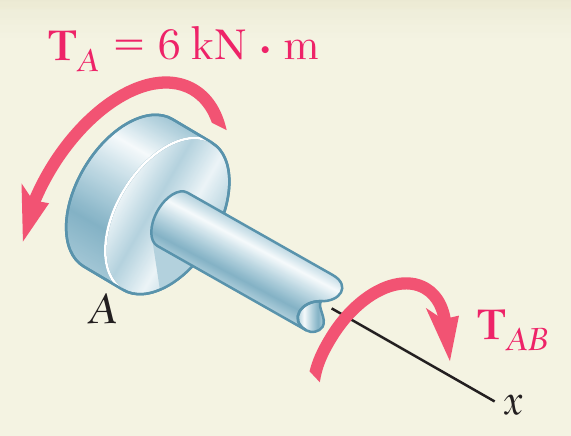
\includegraphics[width=\linewidth,height=2.9cm,keepaspectratio]{Chap_3/sp_3_1_b.png}\\[2pt]
      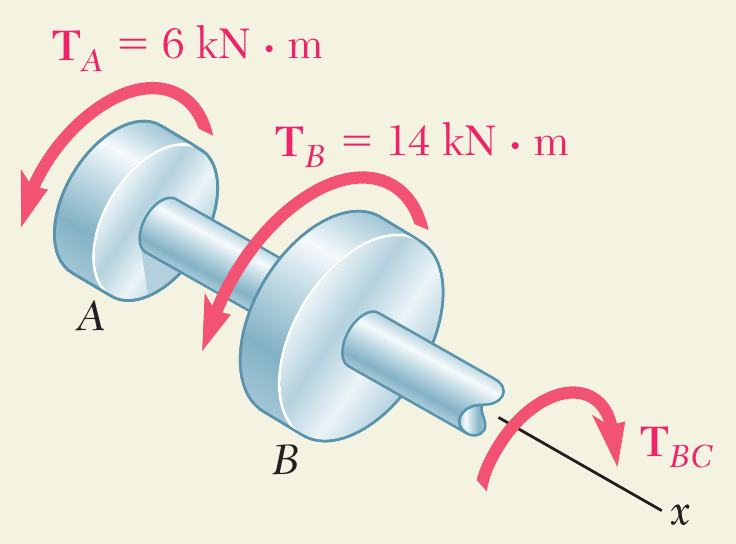
\includegraphics[width=\linewidth,height=2.9cm,keepaspectratio]{Chap_3/sp_3_1_c.png}
  \end{columns}
\end{frame}
% ===========
\begin{frame}[t]{Bài mẫu 3.1 (tiếp)}
  \begin{columns}[T]
    \column{0.52\textwidth}
      \footnotesize
      \begin{itemize}
        \item Áp dụng công thức xoắn đàn hồi để tìm ứng suất nhỏ nhất và
              lớn nhất trong trục $BC$:
      \end{itemize}
      \[
        J = \frac{\pi}{2}\left(c_2^4 - c_1^4\right)
          = \frac{\pi}{2}\left[(0{,}060)^4 - (0{,}045)^4\right]
      \]
      \[
        J = 13{,}92\times10^{-6}\,\mathrm{m}^4
      \]
      \[
        \tau_{\max} = \tau_2 = \frac{T_{BC}c_2}{J}
          = \frac{(20\times10^{3})(0{,}060)}{13{,}92\times10^{-6}}
          = 86{,}2\,\mathrm{MPa}
      \]
      \[
        \frac{\tau_{\min}}{\tau_{\max}} = \frac{c_1}{c_2}
        \;\Rightarrow\;
        \frac{\tau_{\min}}{86{,}2\,\mathrm{MPa}} = \frac{45\,\mathrm{mm}}{60\,\mathrm{mm}}
      \]
      \[
        \boxed{\tau_{\max} = 86{,}2\,\mathrm{MPa}, \quad
               \tau_{\min} = 64{,}7\,\mathrm{MPa}}
      \]
      \centering
      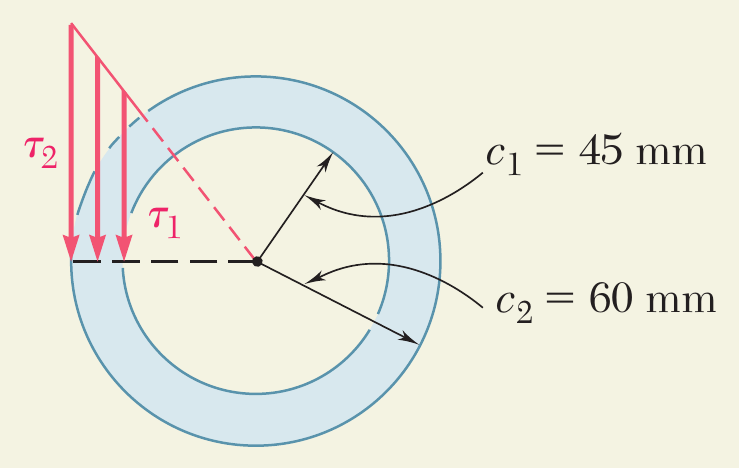
\includegraphics[width=0.6\linewidth,height=1.6cm,keepaspectratio]{Chap_3/sp_3_1_d.png}
    \column{0.46\textwidth}
      \footnotesize
      \begin{itemize}
        \item Với ứng suất tiếp cho phép và mô men xoắn đã biết, giải
              ngược công thức xoắn đàn hồi để tìm đường kính cần thiết:
      \end{itemize}
      \[
        \tau_{\max} = \frac{Tc}{J} = \frac{Tc}{\frac{\pi}{2}c^4}
      \]
      \[
        65\,\mathrm{MPa} = \frac{6\,\mathrm{kN\cdot m}}{\frac{\pi}{2}c^3}
        \;\Rightarrow\;
        c = 38{,}9\times10^{-3}\,\mathrm{m}
      \]
      \[
        \boxed{d = 2c = 77{,}8\,\mathrm{mm}}
      \]
      \centering
      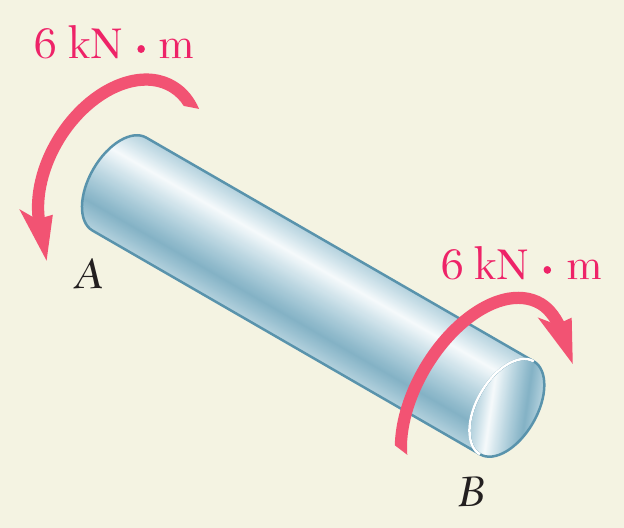
\includegraphics[width=0.8\linewidth,height=2.4cm,keepaspectratio]{Chap_3/sp_3_1_e.png}
  \end{columns}
\end{frame}
% ===========
\section{Góc xoắn trong miền đàn hồi}
\begin{frame}[t]{Góc xoắn trong miền đàn hồi}
  \begin{columns}[T]
    \column{0.58\textwidth}
      \footnotesize
      \begin{itemize}
        \setlength{\itemsep}{0.25em}
        \item Nhắc lại quan hệ giữa góc xoắn và biến dạng trượt lớn nhất:
        \[
          \gamma_{\max} = \frac{c\phi}{L}
        \]
        \item Trong miền đàn hồi, biến dạng trượt và ứng suất tiếp liên hệ
              theo định luật Hooke:
        \[
          \gamma_{\max} = \frac{\tau_{\max}}{G} = \frac{Tc}{JG}
        \]
        \item Cân bằng hai biểu thức của biến dạng trượt và giải ra góc
              xoắn:
        \[
          \phi = \frac{TL}{JG}
        \]
        \item Nếu tải trọng xoắn hoặc mặt cắt ngang thay đổi dọc theo
              chiều dài, góc xoắn bằng tổng góc xoắn của các đoạn:
        \[
          \phi = \sum_i \frac{T_iL_i}{J_iG_i}
        \]
      \end{itemize}
    \column{0.40\textwidth}
      \centering
      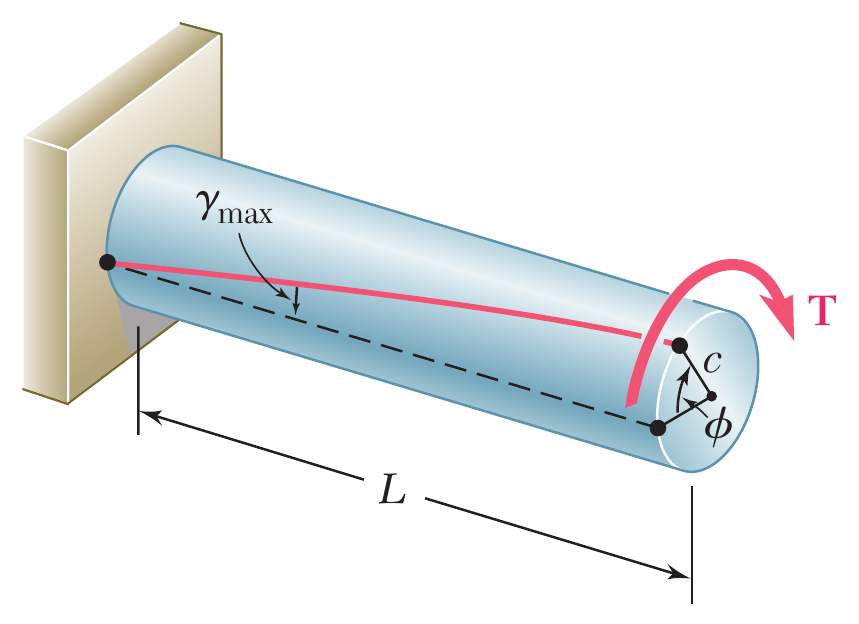
\includegraphics[width=\linewidth,height=2.5cm,keepaspectratio]{Chap_3/fig_3_20.png}\\[2pt]
      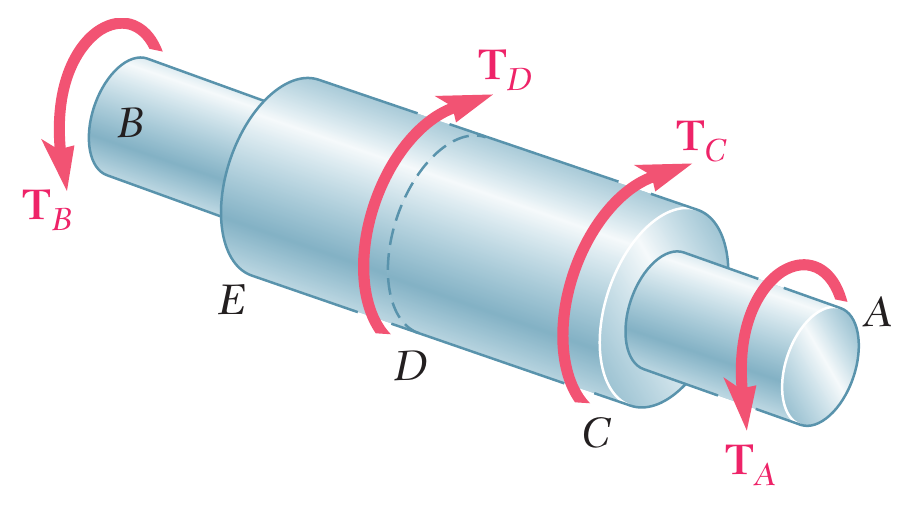
\includegraphics[width=\linewidth,height=2.5cm,keepaspectratio]{Chap_3/fig_3_21.png}
  \end{columns}
\end{frame}
% ===========
\section{Trục siêu tĩnh}
\begin{frame}[t]{Trục siêu tĩnh}
  \begin{columns}[T]
    \column{0.62\textwidth}
      \footnotesize
      \begin{itemize}
        \setlength{\itemsep}{0.5em}
        \item Với kích thước trục và mô men xoắn tác dụng đã biết, cần tìm
              các mô men phản lực tại $A$ và $B$.
        \item Từ phân tích vật thể tự do của trục:
        \[
          T_A + T_B = 120\,\mathrm{N\cdot m}
        \]
        phương trình này không đủ để tìm mô men xoắn tại hai đầu. Bài toán
        là siêu tĩnh.
        \item Chia trục thành hai đoạn phải có biến dạng tương thích:
        \[
          \phi = \phi_1 + \phi_2 = \frac{T_AL_1}{J_1G} - \frac{T_BL_2}{J_2G} = 0
          \qquad
          T_B = \frac{L_1J_2}{L_2J_1}T_A
        \]
        \item Thế vào phương trình cân bằng ban đầu:
        \[
          T_A + \frac{L_1J_2}{L_2J_1}T_A = 120\,\mathrm{N\cdot m}
        \]
      \end{itemize}
    \column{0.36\textwidth}
      \centering
      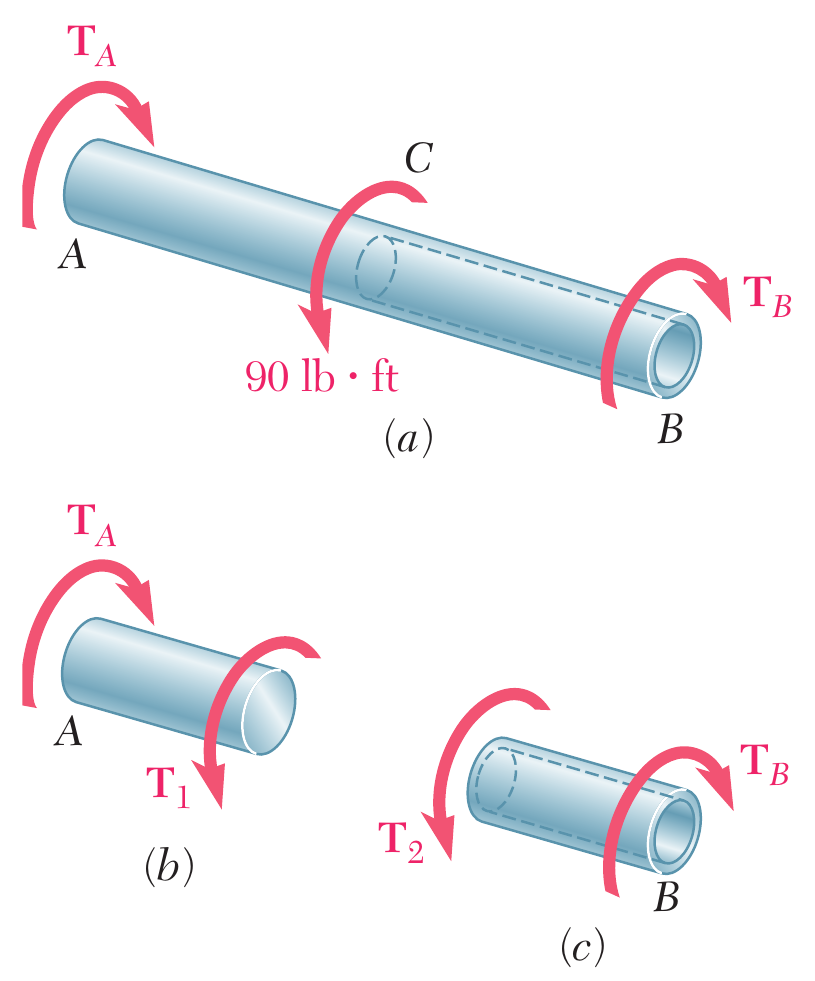
\includegraphics[width=\linewidth,height=5.5cm,keepaspectratio]{Chap_3/fig_3_26.png}
  \end{columns}
\end{frame}
% ===========
\section{Bài mẫu 3.4}
\begin{frame}[t]{Bài mẫu 3.4}
  \begin{columns}[T]
    \column{0.40\textwidth}
      \centering
      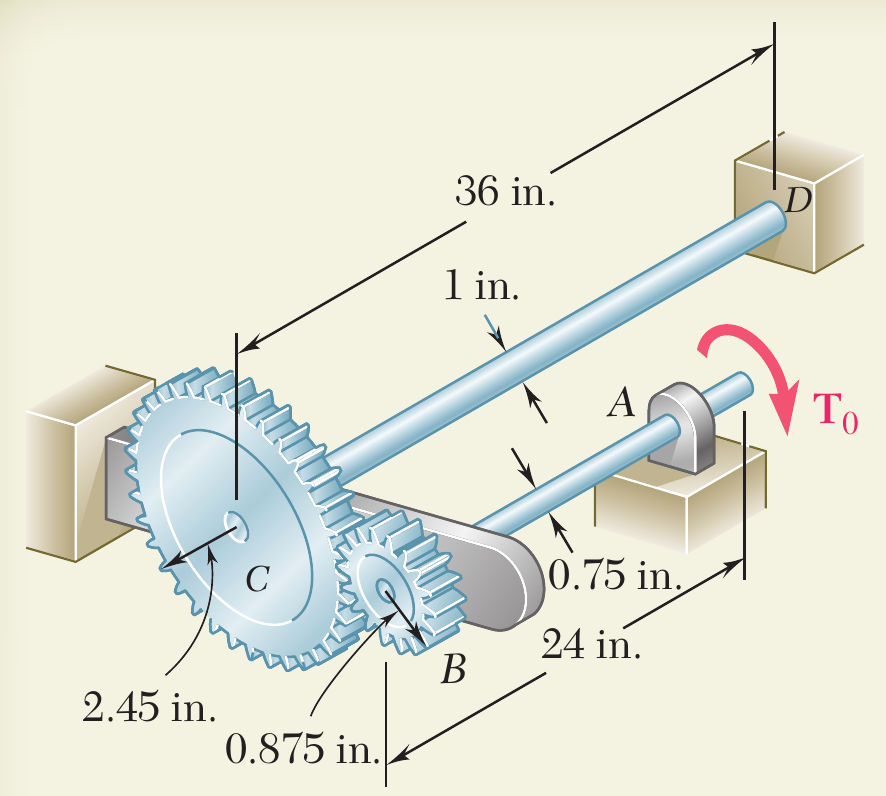
\includegraphics[width=\linewidth,height=5.5cm,keepaspectratio]{Chap_3/sp_3_4_a.png}
    \column{0.58\textwidth}
      \footnotesize
      Hai trục thép đặc được nối với nhau bằng bánh răng. Biết rằng mỗi
      trục có $G = 77\,\mathrm{GPa}$ và ứng suất tiếp cho phép là
      55 MPa, xác định (a) mô men xoắn lớn nhất $T_0$ có thể đặt vào đầu
      trục $AB$, (b) góc xoay tương ứng của đầu $A$ của trục $AB$.

      \vspace{0.5em}
      \textbf{LỜI GIẢI:}
      \begin{itemize}
        \setlength{\itemsep}{0.4em}
        \item Phân tích cân bằng tĩnh học cho hai trục để tìm quan hệ giữa
              $T_{CD}$ và $T_0$.
        \item Phân tích động học để liên hệ góc xoay của các bánh răng.
        \item Tìm mô men xoắn cho phép lớn nhất trên mỗi trục -- chọn giá
              trị nhỏ nhất.
        \item Tìm góc xoắn tương ứng của mỗi trục và góc xoay tổng của đầu
              $A$.
      \end{itemize}
  \end{columns}
\end{frame}
% ===========
\begin{frame}[t]{Bài mẫu 3.4 (tiếp)}
  \begin{columns}[T]
    \column{0.49\textwidth}
      \small
      \begin{itemize}
        \item Phân tích cân bằng tĩnh học cho hai trục để tìm quan hệ giữa
              $T_{CD}$ và $T_0$:
      \end{itemize}
      \[
        \textstyle\sum M_B = 0 = F(22\,\mathrm{mm}) - T_0
      \]
      \[
        \textstyle\sum M_C = 0 = F(60\,\mathrm{mm}) - T_{CD}
      \]
      \[
        T_{CD} = 2{,}73\,T_0
      \]
    \column{0.49\textwidth}
      \small
      \begin{itemize}
        \item Phân tích động học để liên hệ góc xoay của các bánh răng:
      \end{itemize}
      \[
        r_B\phi_B = r_C\phi_C
      \]
      \[
        \phi_B = \frac{r_C}{r_B}\phi_C
          = \frac{60\,\mathrm{mm}}{22\,\mathrm{mm}}\phi_C
      \]
      \[
        \phi_B = 2{,}73\,\phi_C
      \]
  \end{columns}
  \vspace{0.3em}
  \centering
  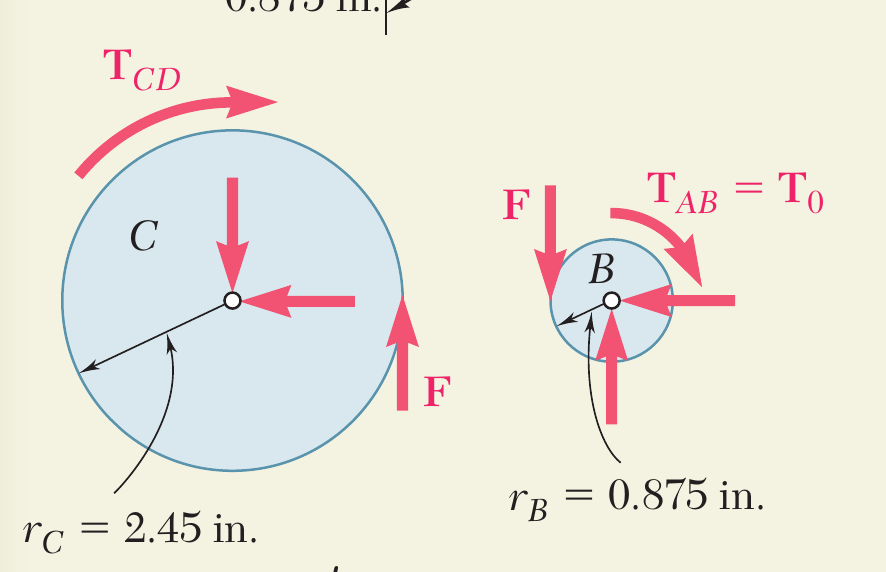
\includegraphics[width=0.6\textwidth,height=2.6cm,keepaspectratio]{Chap_3/sp_3_4_b.png}
\end{frame}
% ===========
\begin{frame}[t]{Bài mẫu 3.4 (tiếp)}
  \begin{columns}[T]
    \column{0.47\textwidth}
      \footnotesize
      \begin{itemize}
        \item Tìm $T_0$ ứng với mô men xoắn cho phép lớn nhất trên mỗi trục
              -- chọn giá trị nhỏ nhất:
      \end{itemize}
      \[
        \tau_{\max} = \frac{T_{AB}c}{J_{AB}}:\quad
        55\times10^{6} = \frac{T_0(9{,}5\times10^{-3})}
                 {\frac{\pi}{2}(9{,}5\times10^{-3})^4}
      \]
      \[ T_0 = 74{,}1\,\mathrm{N\cdot m} \]
      \[
        \tau_{\max} = \frac{T_{CD}c}{J_{CD}}:\quad
        55\times10^{6} = \frac{2{,}73\,T_0(12{,}5\times10^{-3})}
                 {\frac{\pi}{2}(12{,}5\times10^{-3})^4}
      \]
      \[ T_0 = 61{,}8\,\mathrm{N\cdot m}
         \qquad \boxed{T_0 = 61{,}8\,\mathrm{N\cdot m}} \]
      \centering
      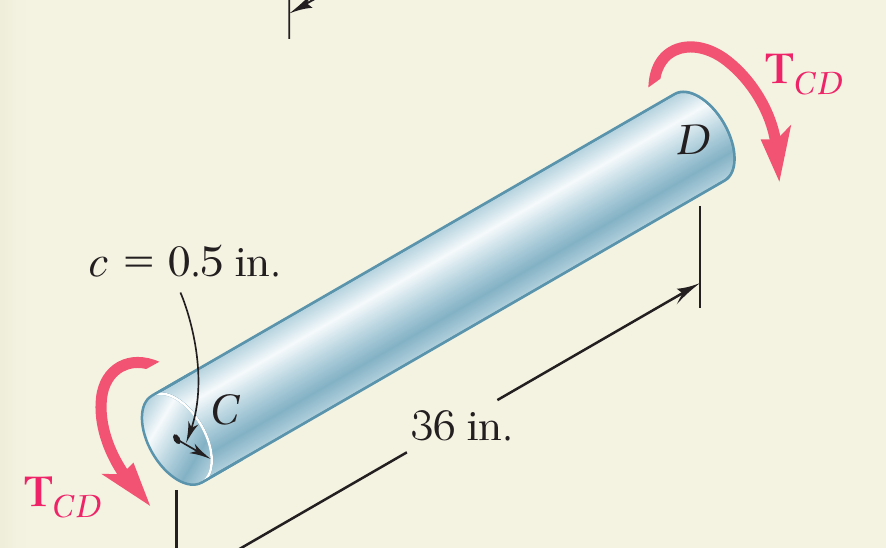
\includegraphics[width=0.7\linewidth,height=1.8cm,keepaspectratio]{Chap_3/sp_3_4_c.png}
    \column{0.51\textwidth}
      \footnotesize
      \begin{itemize}
        \item Tìm góc xoắn tương ứng của mỗi trục và góc xoay tổng của đầu
              $A$:
      \end{itemize}
      \[
        \phi_{A/B} = \frac{T_{AB}L}{J_{AB}G}
          = \frac{(61{,}8)(0{,}6)}{\frac{\pi}{2}(0{,}0095)^4(77\times10^{9})}
      \]
      \[
        \phi_{A/B} = 0{,}0376\,\mathrm{rad} = 2{,}15^\circ
      \]
      \[
        \phi_{C/D} = \frac{T_{CD}L}{J_{CD}G}
          = \frac{2{,}73(61{,}8)(0{,}6)}{\frac{\pi}{2}(0{,}0125)^4(77\times10^{9})}
      \]
      \[
        \phi_{C/D} = 0{,}0514\,\mathrm{rad} = 2{,}95^\circ
      \]
      \[
        \phi_B = 2{,}73\,\phi_C = 2{,}73(2{,}95^\circ) = 8{,}05^\circ
      \]
      \[
        \phi_A = \phi_B + \phi_{A/B} = 8{,}05^\circ + 2{,}15^\circ
        \qquad \boxed{\phi_A = 10{,}2^\circ}
      \]
      \centering
      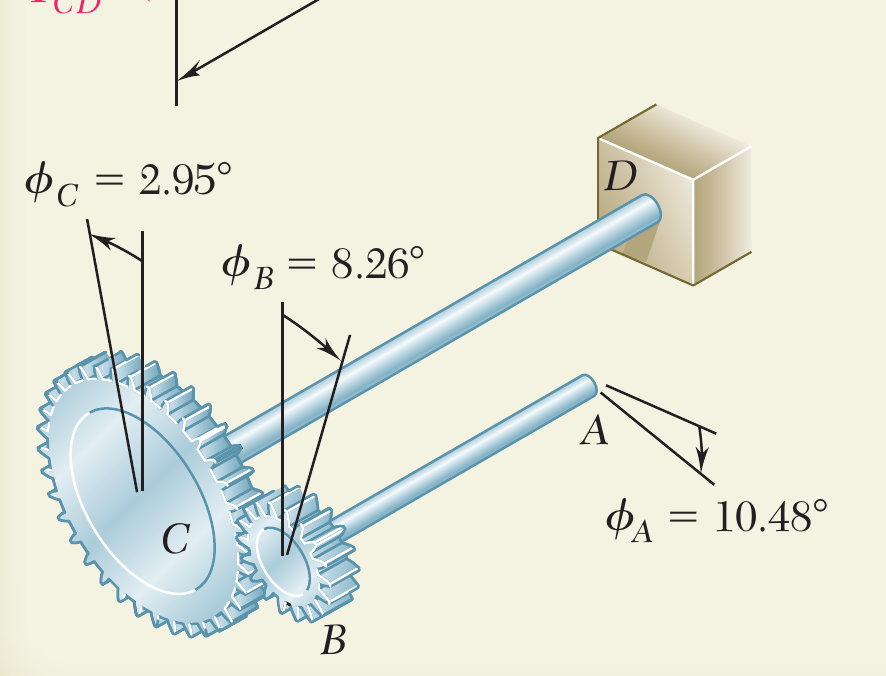
\includegraphics[width=0.6\linewidth,height=1.5cm,keepaspectratio]{Chap_3/sp_3_4_d.png}
  \end{columns}
\end{frame}
% ===========
\section{Thiết kế trục truyền động}
\begin{frame}[t]{Thiết kế trục truyền động}
  \begin{columns}[T]
    \column{0.48\textwidth}
      \small
      \begin{itemize}
        \setlength{\itemsep}{0.8em}
        \item Các thông số làm việc chủ yếu của trục truyền động là:
              \begin{itemize}
                \item công suất
                \item tốc độ quay
              \end{itemize}
        \item Người thiết kế phải chọn vật liệu và mặt cắt ngang của trục
              để đáp ứng các thông số làm việc mà không vượt quá ứng suất
              tiếp cho phép.
      \end{itemize}
    \column{0.50\textwidth}
      \small
      \begin{itemize}
        \setlength{\itemsep}{0.6em}
        \item Xác định mô men xoắn tác dụng lên trục ứng với công suất và
              tốc độ cho trước:
        \[
          P = T\omega = 2\pi fT
          \qquad
          T = \frac{P}{\omega} = \frac{P}{2\pi f}
        \]
        \item Tìm mặt cắt ngang của trục sao cho không vượt quá ứng suất
              tiếp cho phép:
        \[
          \tau_{\max} = \frac{Tc}{J}
        \]
        \[
          \frac{J}{c} = \frac{\pi}{2}c^3 = \frac{T}{\tau_{\max}}
          \quad\text{(trục đặc)}
        \]
        \[
          \frac{J}{c_2} = \frac{\pi}{2c_2}\left(c_2^4 - c_1^4\right)
            = \frac{T}{\tau_{\max}}
          \quad\text{(trục rỗng)}
        \]
      \end{itemize}
  \end{columns}
\end{frame}
% ===========
\section{Tập trung ứng suất}
\begin{frame}[t]{Tập trung ứng suất}
  \begin{columns}[T]
    \column{0.56\textwidth}
      \small
      \begin{itemize}
        \setlength{\itemsep}{0.6em}
        \item Khi thiết lập công thức xoắn
              \[ \tau_{\max} = \frac{Tc}{J} \]
              ta đã giả thiết trục tròn có mặt cắt ngang không đổi, chịu
              tải qua các tấm cứng ở hai đầu.
        \item Việc dùng khớp nối mặt bích, bánh răng và puli lắp trên trục
              bằng then trong rãnh then, cũng như sự thay đổi đột ngột của
              mặt cắt ngang, có thể gây ra tập trung ứng suất.
        \item Hệ số tập trung ứng suất xác định bằng thực nghiệm hoặc tính
              số được áp dụng như sau:
              \[ \tau_{\max} = K\frac{Tc}{J} \]
      \end{itemize}
    \column{0.42\textwidth}
      \centering
      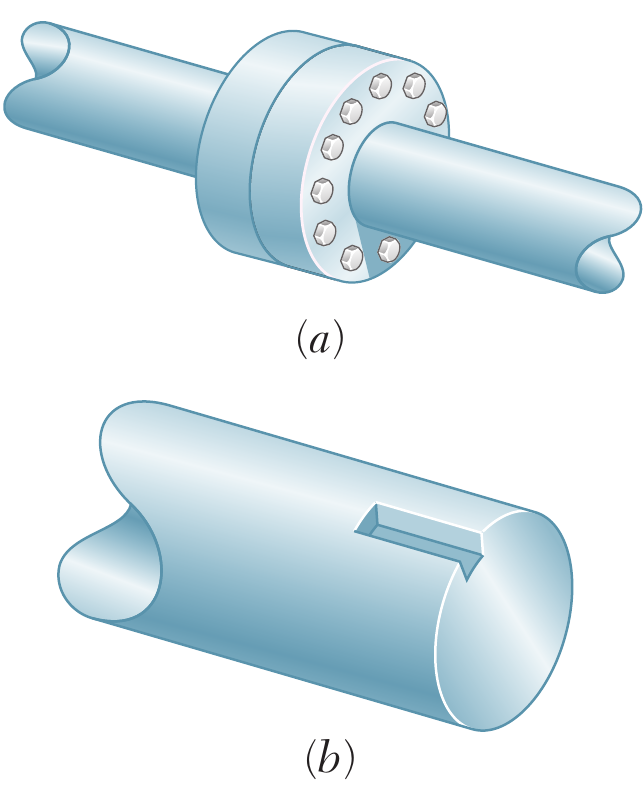
\includegraphics[width=\linewidth,height=2.4cm,keepaspectratio]{Chap_3/fig_3_27.png}\\[2pt]
      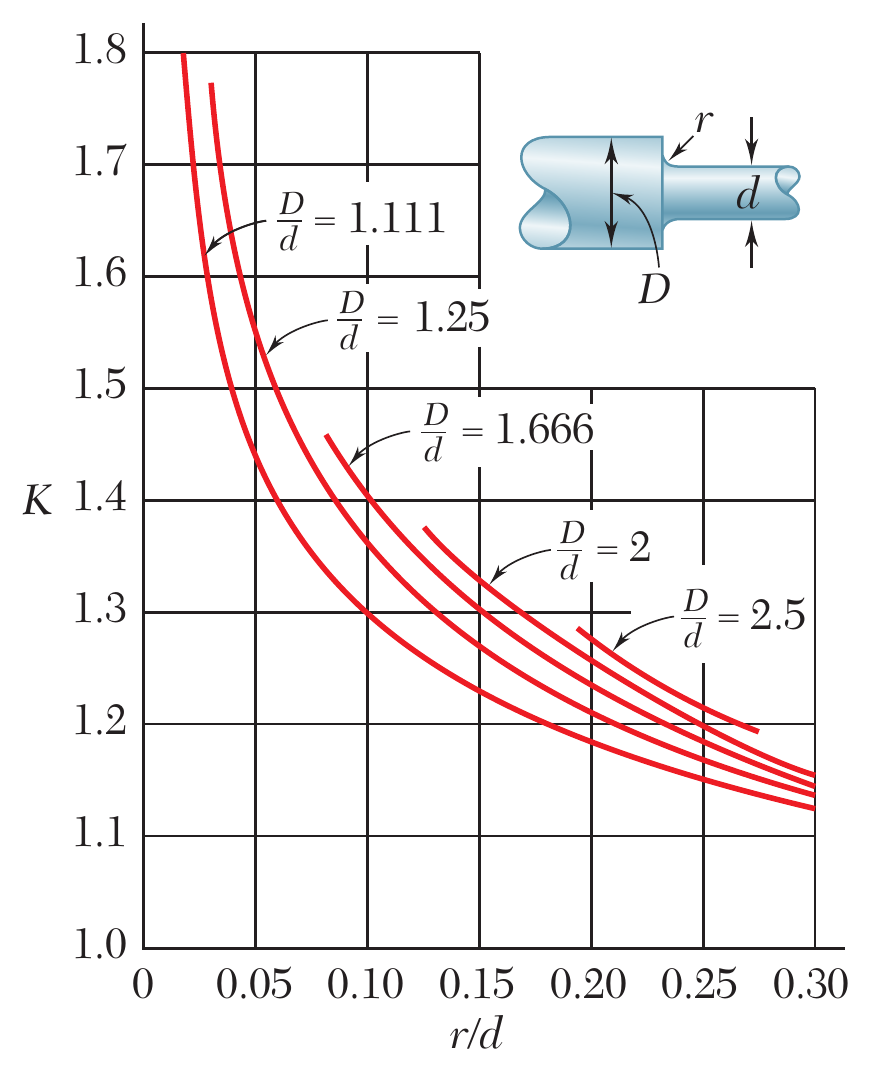
\includegraphics[width=\linewidth,height=3.0cm,keepaspectratio]{Chap_3/fig_3_29.png}\\
      \scriptsize Hình 3.32: Hệ số tập trung ứng suất tại góc lượn của
      trục tròn.
  \end{columns}
\end{frame}
% ===========
\section{Biến dạng dẻo}
\begin{frame}[t]{Biến dạng dẻo}
  \begin{columns}[T]
    \column{0.60\textwidth}
      \small
      \begin{itemize}
        \setlength{\itemsep}{0.5em}
        \item Với giả thiết vật liệu đàn hồi tuyến tính:
        \[
          \tau_{\max} = \frac{Tc}{J}
        \]
        \item Nếu vượt quá giới hạn chảy hoặc vật liệu có đường cong ứng
              suất tiếp -- biến dạng trượt phi tuyến, biểu thức này không
              còn đúng.
        \item Biến dạng trượt vẫn thay đổi tuyến tính bất kể tính chất vật
              liệu. Áp dụng đường cong ứng suất tiếp -- biến dạng trượt cho
              phép xác định phân bố ứng suất.
        \item Tích phân mô men của phân bố nội ứng suất bằng mô men xoắn
              của trục tại mặt cắt:
        \[
          T = \int_0^c \rho\,\tau\,(2\pi\rho\,d\rho)
            = 2\pi\int_0^c \rho^2\tau\,d\rho
        \]
      \end{itemize}
    \column{0.38\textwidth}
      \centering
      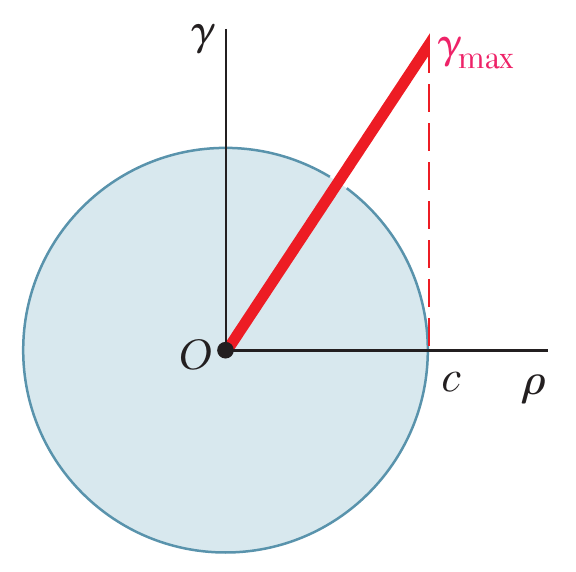
\includegraphics[width=\linewidth,height=1.9cm,keepaspectratio]{Chap_3/fig_3_30.png}\\[2pt]
      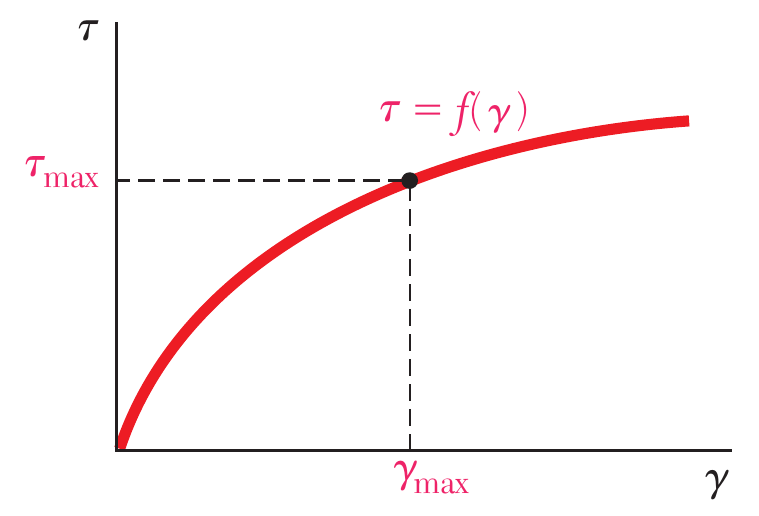
\includegraphics[width=\linewidth,height=1.9cm,keepaspectratio]{Chap_3/fig_3_31.png}\\[2pt]
      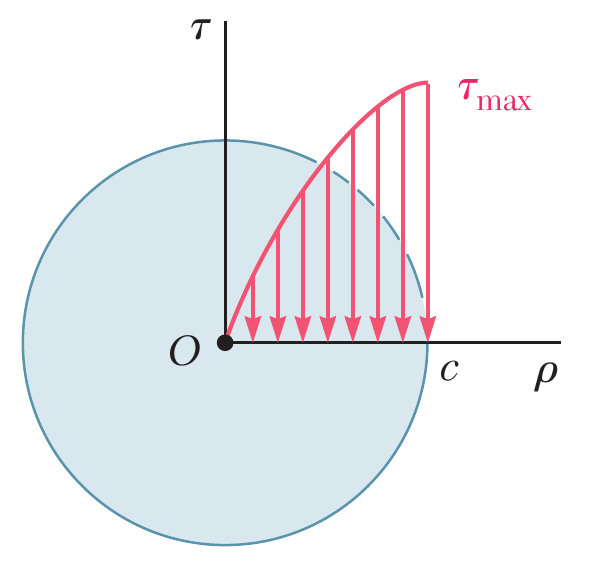
\includegraphics[width=\linewidth,height=1.9cm,keepaspectratio]{Chap_3/fig_3_32.png}
  \end{columns}
\end{frame}
% ===========
\section{Vật liệu đàn -- dẻo}
\begin{frame}[t]{Vật liệu đàn -- dẻo}
  \begin{columns}[T]
    \column{0.62\textwidth}
      \footnotesize
      \begin{itemize}
        \setlength{\itemsep}{0.4em}
        \item Tại mô men xoắn đàn hồi lớn nhất:
        \[
          T_Y = \frac{J}{c}\tau_Y = \tfrac{1}{2}\pi c^3\tau_Y
          \qquad
          \phi_Y = \frac{L\gamma_Y}{c}
        \]
        \item Khi mô men xoắn tăng, một vùng dẻo ($\tau = \tau_Y$) hình
              thành bao quanh lõi đàn hồi ($\tau = \frac{\rho}{\rho_Y}\tau_Y$):
        \[
          T = \tfrac{2}{3}\pi c^3\tau_Y\left(1 - \tfrac{1}{4}\frac{\rho_Y^3}{c^3}\right)
            = \tfrac{4}{3}T_Y\left(1 - \tfrac{1}{4}\frac{\rho_Y^3}{c^3}\right)
        \]
        \[
          \rho_Y = \frac{L\gamma_Y}{\phi}
          \qquad
          T = \tfrac{4}{3}T_Y\left(1 - \tfrac{1}{4}\frac{\phi_Y^3}{\phi^3}\right)
        \]
        \item Khi $\rho_Y \to 0$, mô men xoắn tiến tới một giá trị giới hạn:
        \[
          T_P = \tfrac{4}{3}T_Y = \text{mô men xoắn dẻo}
        \]
      \end{itemize}
    \column{0.36\textwidth}
      \centering
      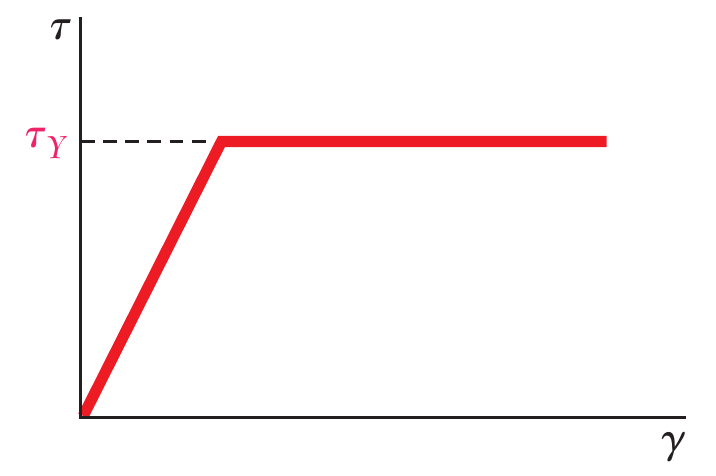
\includegraphics[width=\linewidth,height=1.4cm,keepaspectratio]{Chap_3/fig_3_34.png}\\[2pt]
      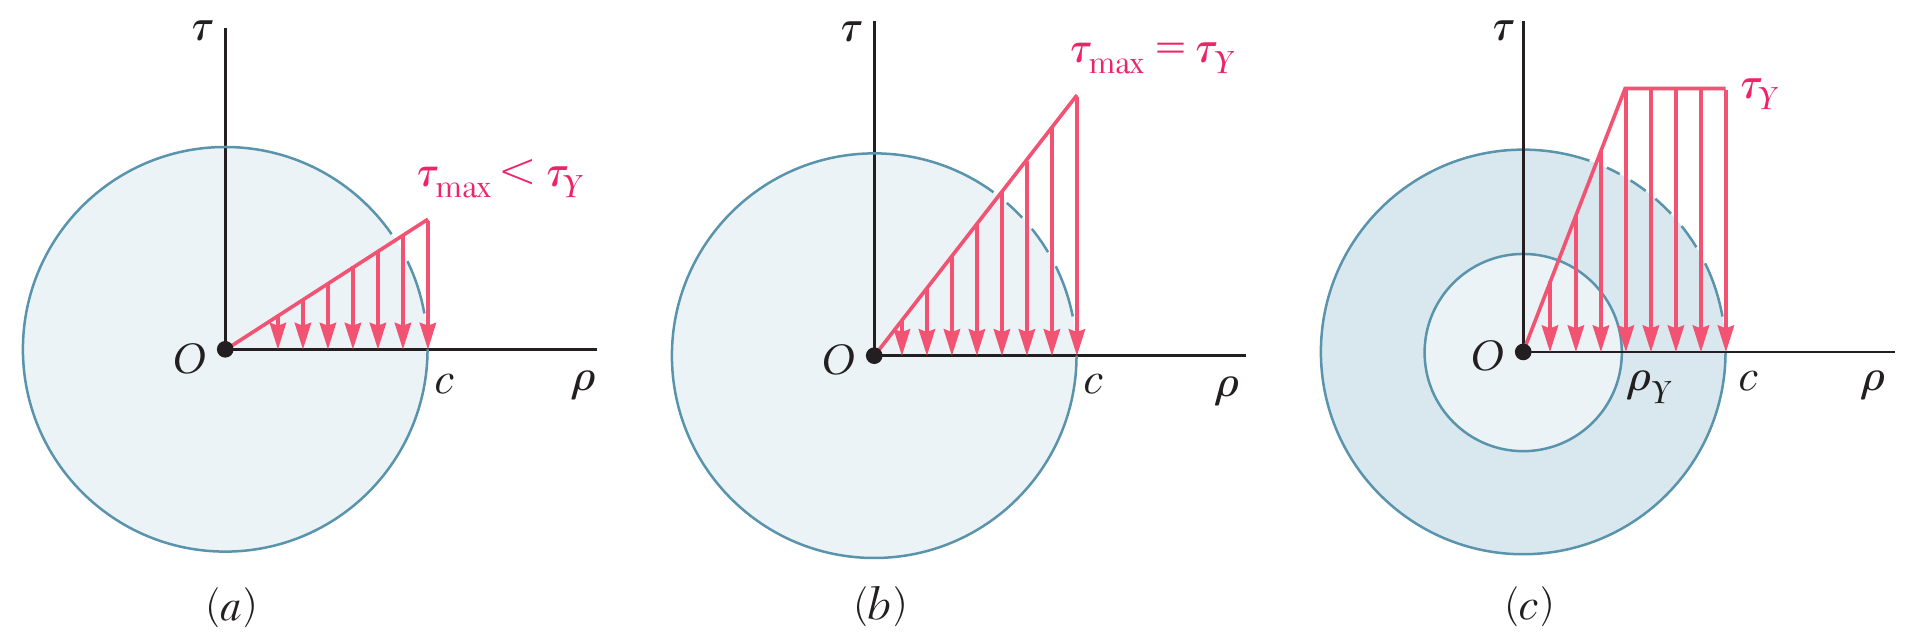
\includegraphics[width=\linewidth,height=1.4cm,keepaspectratio]{Chap_3/fig_3_35.png}\\[2pt]
      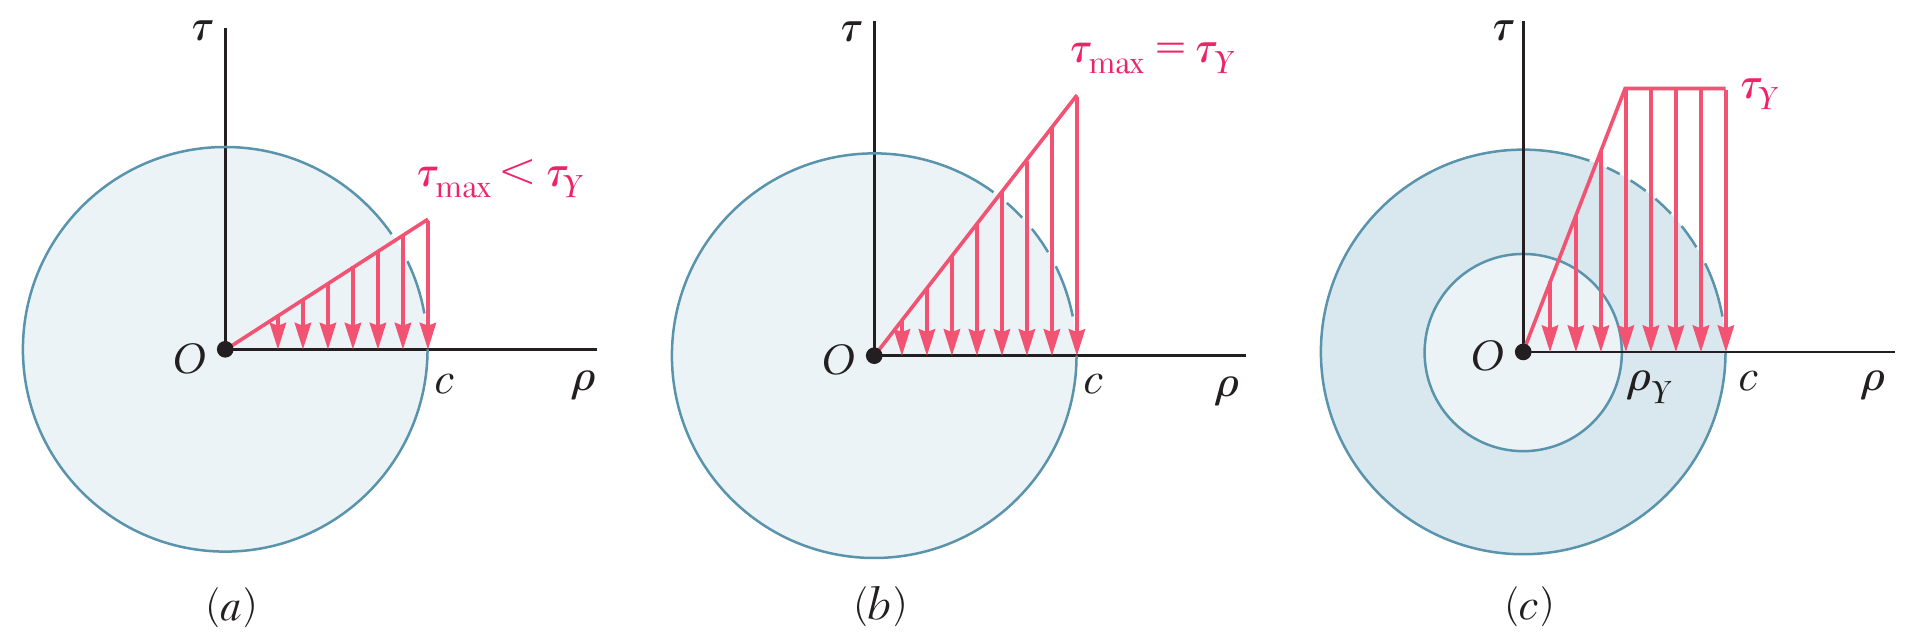
\includegraphics[width=\linewidth,height=1.4cm,keepaspectratio]{Chap_3/fig_3_35.png}\\[2pt]
      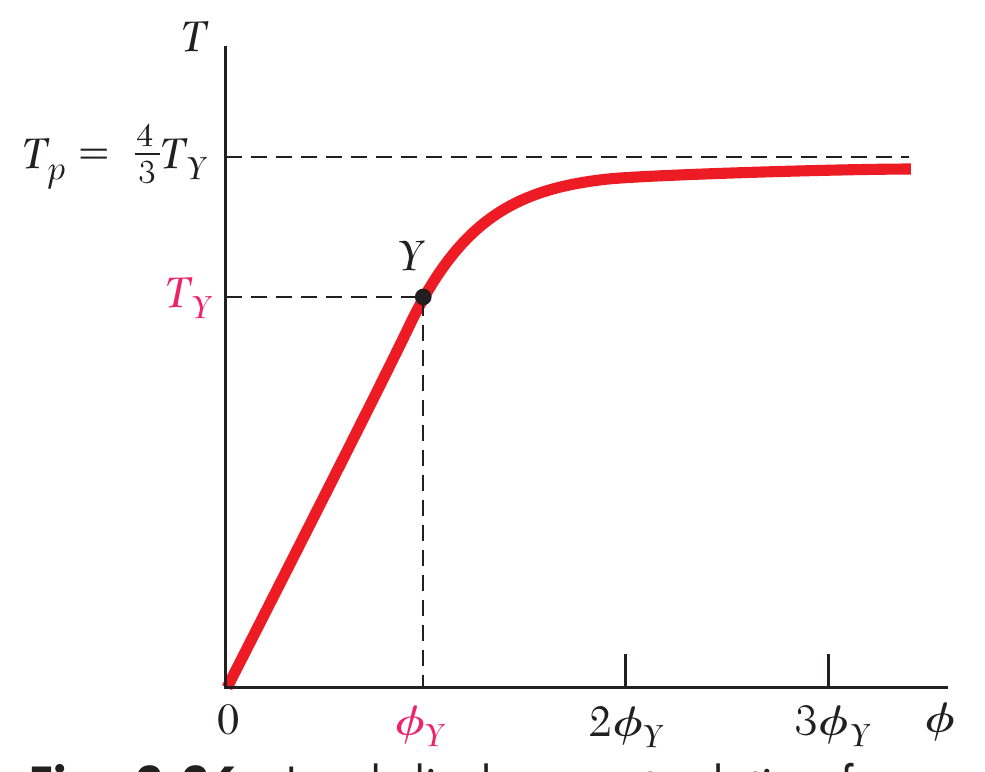
\includegraphics[width=\linewidth,height=1.4cm,keepaspectratio]{Chap_3/fig_3_36.png}
  \end{columns}
\end{frame}
% ===========
\section{Ứng suất dư}
\begin{frame}[t]{Ứng suất dư}
  \begin{columns}[T]
    \column{0.58\textwidth}
      \small
      \begin{itemize}
        \setlength{\itemsep}{0.6em}
        \item Vùng dẻo hình thành trong trục khi chịu mô men xoắn đủ lớn.
        \item Khi bỏ mô men xoắn, sự giảm ứng suất và biến dạng tại mỗi
              điểm diễn ra theo một đường thẳng, dẫn tới một ứng suất dư
              nói chung khác không.
        \item Trên đường cong $T$--$\phi$, trục dỡ tải theo một đường thẳng
              về một góc lớn hơn không.
        \item Ứng suất dư được xác định theo nguyên lý cộng tác dụng:
        \[
          \tau'_m = \frac{Tc}{J}
          \qquad
          \int \rho(\tau\,dA) = 0
        \]
      \end{itemize}
    \column{0.40\textwidth}
      \centering
      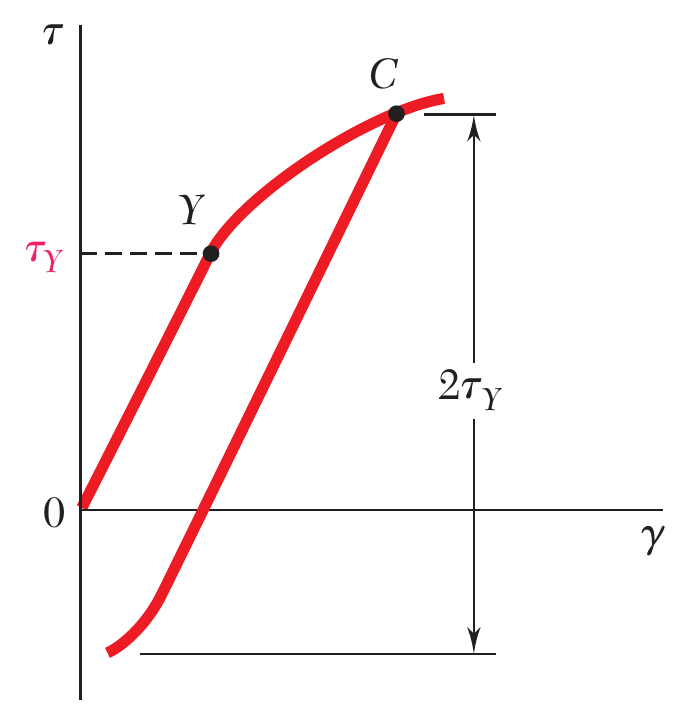
\includegraphics[width=\linewidth,height=1.9cm,keepaspectratio]{Chap_3/fig_3_38.png}\\[2pt]
      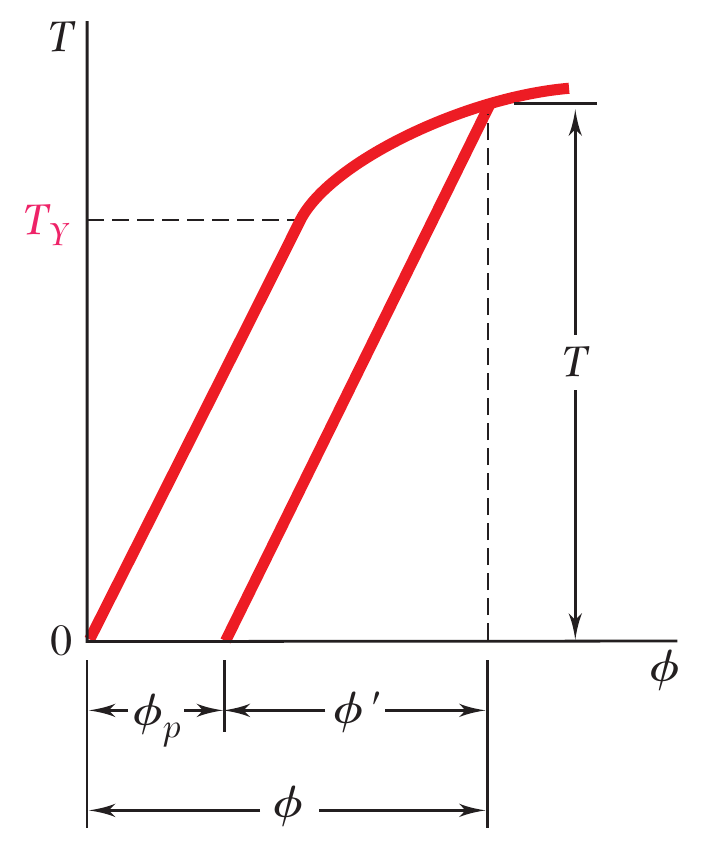
\includegraphics[width=\linewidth,height=1.9cm,keepaspectratio]{Chap_3/fig_3_39.png}\\[2pt]
      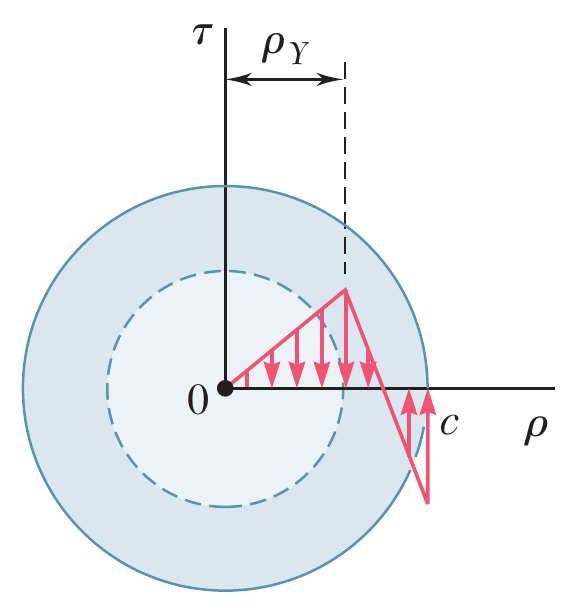
\includegraphics[width=\linewidth,height=1.9cm,keepaspectratio]{Chap_3/ex_3_09.png}
  \end{columns}
\end{frame}
% ===========
\section{Ví dụ 3.08/3.09}
\begin{frame}[t]{Ví dụ 3.08/3.09}
  \begin{columns}[T]
    \column{0.40\textwidth}
      \centering
      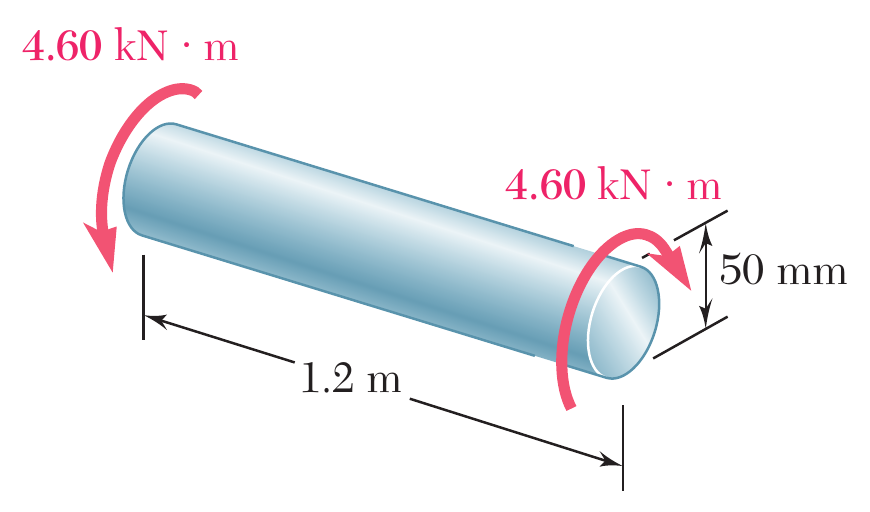
\includegraphics[width=\linewidth,height=5.5cm,keepaspectratio]{Chap_3/fig_3_37.png}
    \column{0.58\textwidth}
      \footnotesize
      Một trục tròn đặc chịu mô men xoắn $T = 4{,}6\,\mathrm{kN\cdot m}$
      ở mỗi đầu. Giả thiết trục làm bằng vật liệu đàn -- dẻo với
      $\tau_Y = 150\,\mathrm{MPa}$ và $G = 77\,\mathrm{GPa}$, xác định
      (a) bán kính lõi đàn hồi, (b) góc xoắn của trục. Khi bỏ mô men xoắn,
      xác định (c) góc xoắn dư, (d) phân bố ứng suất dư.

      \vspace{0.5em}
      \textbf{LỜI GIẢI:}
      \begin{itemize}
        \setlength{\itemsep}{0.3em}
        \item Giải phương trình (3.32) để tìm $\rho_Y/c$ và tính bán kính
              lõi đàn hồi.
        \item Giải phương trình (3.36) để tìm góc xoắn.
        \item Tính theo phương trình (3.16) góc mà trục xoắn ngược lại khi
              bỏ mô men. Góc xoắn dư là hiệu giữa góc xoắn và góc xoắn
              ngược.
        \item Tìm phân bố ứng suất dư bằng cách cộng tác dụng ứng suất do
              xoắn và do xoắn ngược trục.
      \end{itemize}
  \end{columns}
\end{frame}
% ===========
\begin{frame}[t]{Ví dụ 3.08/3.09 (tiếp)}
  \begin{columns}[T]
    \column{0.49\textwidth}
      \footnotesize
      \begin{itemize}
        \item Giải phương trình (3.32) để tìm $\rho_Y/c$ và tính bán kính
              lõi đàn hồi:
      \end{itemize}
      \[
        T = \tfrac{4}{3}T_Y\left(1 - \tfrac{1}{4}\frac{\rho_Y^3}{c^3}\right)
        \;\Rightarrow\;
        \frac{\rho_Y}{c} = \left(4 - 3\frac{T}{T_Y}\right)^{1/3}
      \]
      \[
        J = \tfrac{1}{2}\pi c^4 = \tfrac{1}{2}\pi(25\times10^{-3})^4
          = 614\times10^{-9}\,\mathrm{m}^4
      \]
      \[
        T_Y = \frac{\tau_Y J}{c}
          = \frac{(150\times10^{6})(614\times10^{-9})}{25\times10^{-3}}
      \]
      \[
        T_Y = 3{,}68\,\mathrm{kN\cdot m}
      \]
      \[
        \frac{\rho_Y}{c} = \left(4 - 3\frac{4{,}6}{3{,}68}\right)^{1/3} = 0{,}630
      \]
      \[
        \boxed{\rho_Y = 15{,}8\,\mathrm{mm}}
      \]
    \column{0.49\textwidth}
      \footnotesize
      \begin{itemize}
        \item Giải phương trình (3.36) để tìm góc xoắn:
      \end{itemize}
      \[
        \frac{\phi}{\phi_Y} = \frac{c}{\rho_Y}
        \;\Rightarrow\;
        \phi = \frac{\phi_Y}{\rho_Y/c}
      \]
      \[
        \phi_Y = \frac{T_YL}{JG}
          = \frac{(3{,}68\times10^{3})(1{,}2)}{(614\times10^{-9})(77\times10^{9})}
          = 93{,}4\times10^{-3}\,\mathrm{rad}
      \]
      \[
        \phi = \frac{93{,}4\times10^{-3}\,\mathrm{rad}}{0{,}630}
          = 148{,}3\times10^{-3}\,\mathrm{rad} = 8{,}50^\circ
      \]
      \[
        \boxed{\phi = 8{,}50^\circ}
      \]
      \centering
  \end{columns}
\end{frame}
% ===========
\begin{frame}[t]{Ví dụ 3.08/3.09 (tiếp)}
  \begin{columns}[T]
    \column{0.56\textwidth}
      \footnotesize
      \begin{itemize}
        \setlength{\itemsep}{0.4em}
        \item Tính theo phương trình (3.16) góc xoắn ngược khi bỏ mô men.
              Góc xoắn dư là hiệu giữa góc xoắn và góc xoắn ngược:
        \[
          \phi' = \frac{TL}{JG}
            = \frac{(4{,}6\times10^{3})(1{,}2)}{(614\times10^{-9})(77\times10^{9})}
        \]
        \[
          \phi' = 116{,}8\times10^{-3}\,\mathrm{rad} = 6{,}69^\circ
        \]
        \[
          \phi_p = \phi - \phi' = 8{,}50^\circ - 6{,}69^\circ = 1{,}81^\circ
          \qquad \boxed{\phi_p = 1{,}81^\circ}
        \]
        \item Tìm phân bố ứng suất dư bằng cách cộng tác dụng ứng suất do
              xoắn và do xoắn ngược trục:
        \[
          \tau'_{\max} = \frac{Tc}{J}
            = \frac{(4{,}6\times10^{3})(25\times10^{-3})}{614\times10^{-9}}
            = 187{,}3\,\mathrm{MPa}
        \]
      \end{itemize}
    \column{0.42\textwidth}
      \centering
      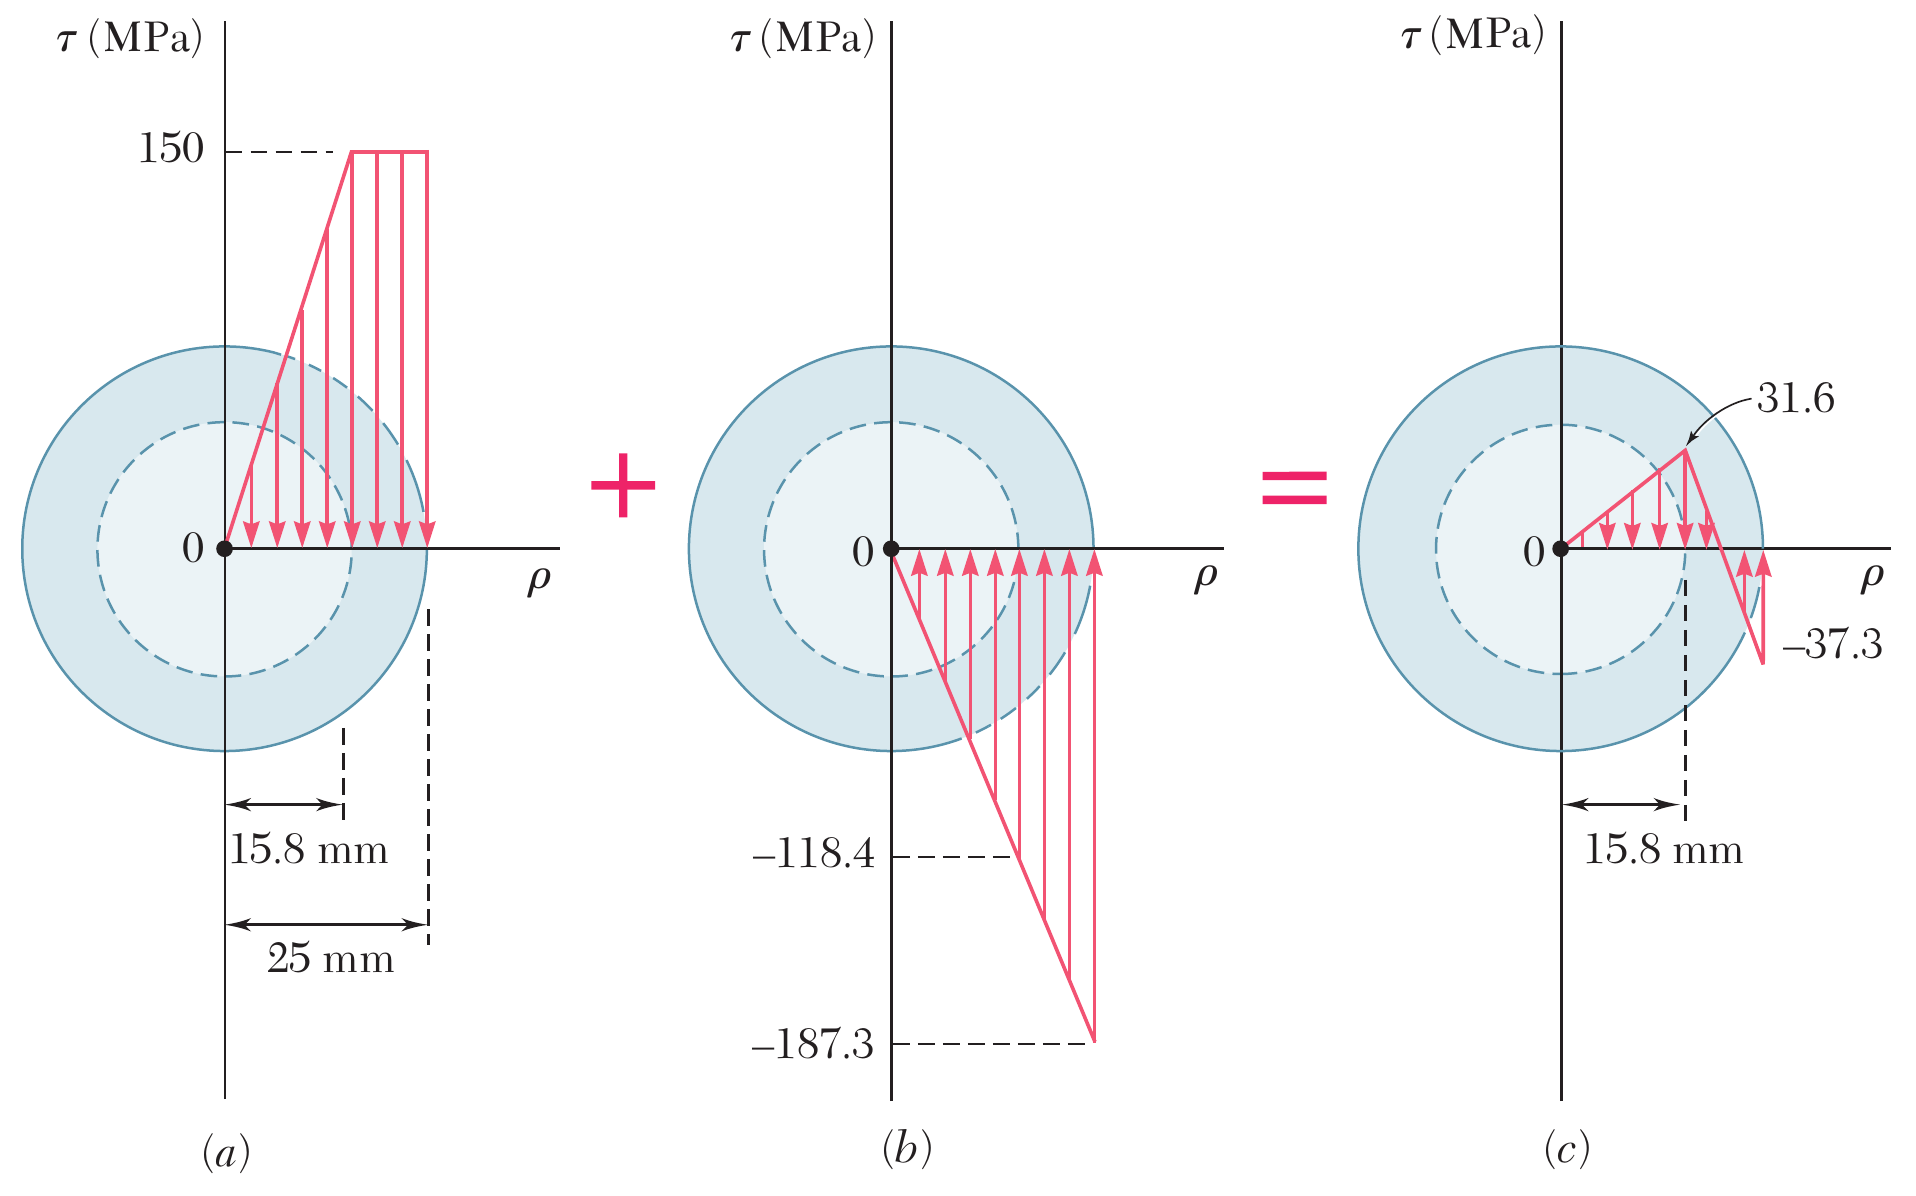
\includegraphics[width=\linewidth,height=5.5cm,keepaspectratio]{Chap_3/fig_3_41.png}
  \end{columns}
\end{frame}
% ===========
\section{Xoắn thanh có mặt cắt không tròn}
\begin{frame}[t]{Xoắn thanh có mặt cắt không tròn}
  \begin{columns}[T]
    \column{0.58\textwidth}
      \small
      \begin{itemize}
        \setlength{\itemsep}{0.6em}
        \item Các công thức xoắn ở trên chỉ đúng cho trục tròn hoặc trục
              đối xứng trục.
        \item Mặt cắt phẳng của trục không tròn không còn phẳng sau biến
              dạng, và phân bố ứng suất, biến dạng không thay đổi tuyến
              tính.
        \item Với mặt cắt chữ nhật không đổi:
        \[
          \tau_{\max} = \frac{T}{c_1ab^2}
          \qquad
          \phi = \frac{TL}{c_2ab^3G}
        \]
        \item Khi tỉ số $a/b$ lớn, ứng suất tiếp lớn nhất và góc xoắn của
              các mặt cắt hở khác cũng giống như của thanh chữ nhật.
      \end{itemize}
    \column{0.40\textwidth}
      \centering
      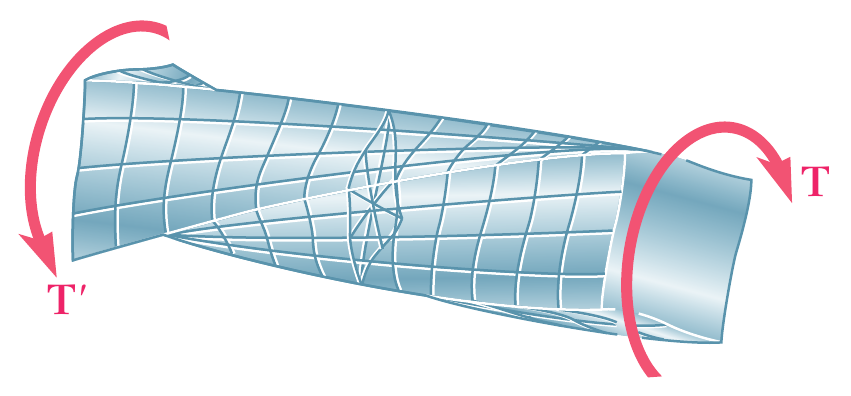
\includegraphics[width=\linewidth,height=1.9cm,keepaspectratio]{Chap_3/fig_3_42.png}\\[2pt]
      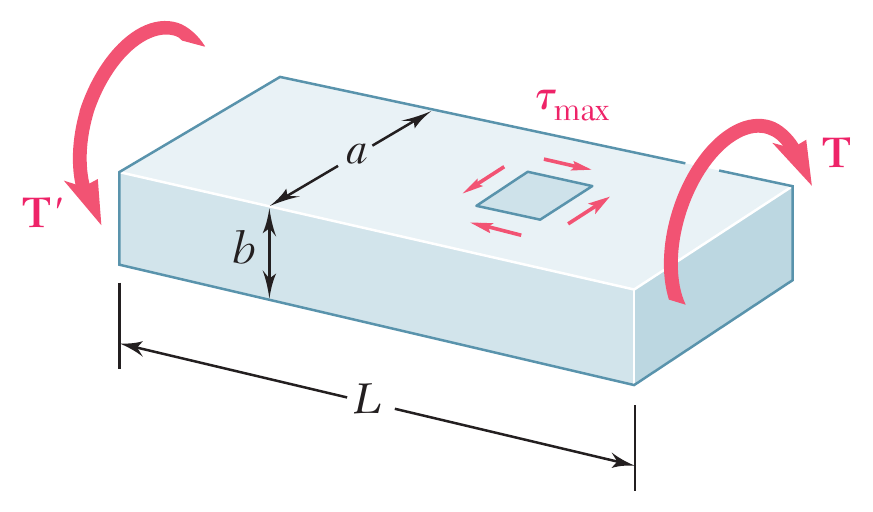
\includegraphics[width=\linewidth,height=1.9cm,keepaspectratio]{Chap_3/fig_3_45.png}\\[2pt]
      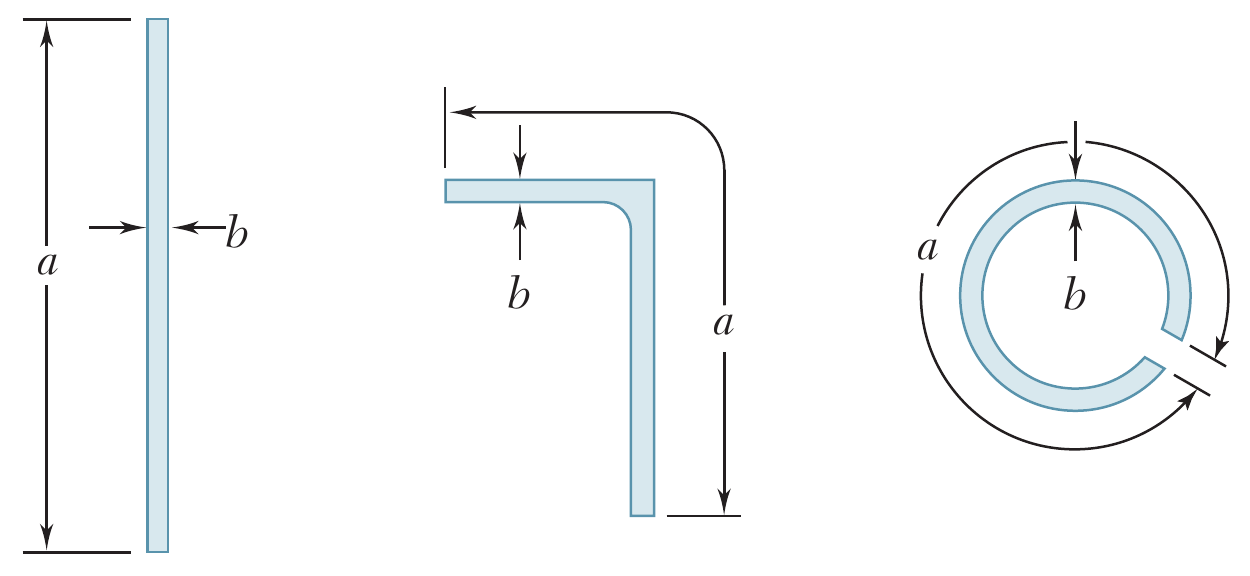
\includegraphics[width=\linewidth,height=1.9cm,keepaspectratio]{Chap_3/fig_3_47.png}
  \end{columns}
\end{frame}
% ===========
\section{Trục rỗng thành mỏng}
\begin{frame}[t]{Trục rỗng thành mỏng}
  \begin{columns}[T]
    \column{0.60\textwidth}
      \footnotesize
      \begin{itemize}
        \setlength{\itemsep}{0.4em}
        \item Tổng hợp các lực theo phương $x$ trên đoạn $AB$:
        \[
          \textstyle\sum F_x = 0 = \tau_A(t_A\Delta x) - \tau_B(t_B\Delta x)
        \]
        \[
          \tau_At_A = \tau_Bt_B = \tau t = q = \text{dòng lực cắt}
        \]
        ứng suất tiếp tỉ lệ nghịch với chiều dày thành.
        \item Tính mô men xoắn của trục từ tích phân mô men do ứng suất
              tiếp:
        \[
          dM_0 = p\,dF = p\,\tau(t\,ds) = q(p\,ds) = 2q\,d\mathcal{A}
        \]
        \[
          T = \oint dM_0 = \oint 2q\,d\mathcal{A} = 2q\mathcal{A}
          \qquad
          \tau = \frac{T}{2t\mathcal{A}}
        \]
        \item Góc xoắn (xem Chương 11):
        \[
          \phi = \frac{TL}{4\mathcal{A}^2G}\oint\frac{ds}{t}
        \]
      \end{itemize}
    \column{0.38\textwidth}
      \centering
      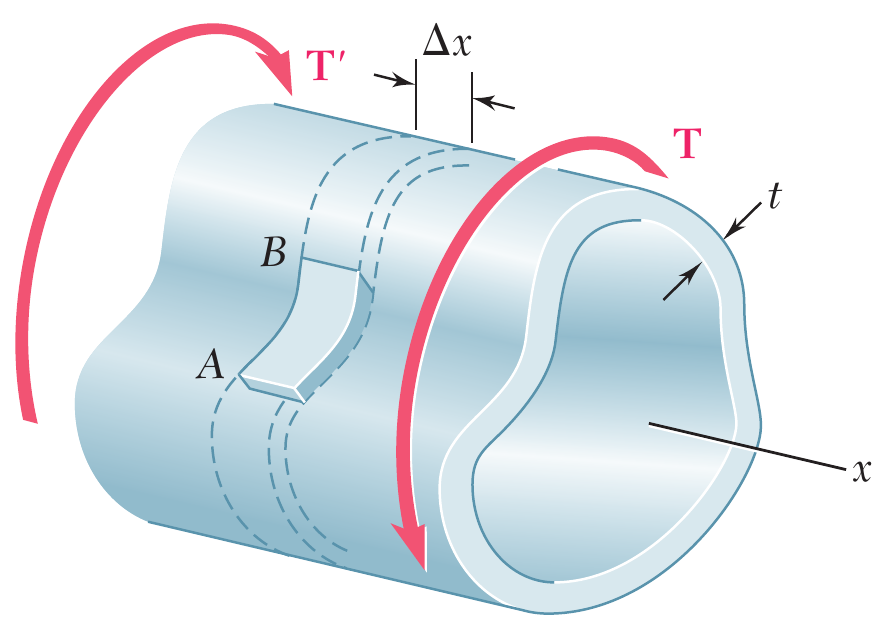
\includegraphics[width=\linewidth,height=1.4cm,keepaspectratio]{Chap_3/fig_3_48.png}\\[2pt]
      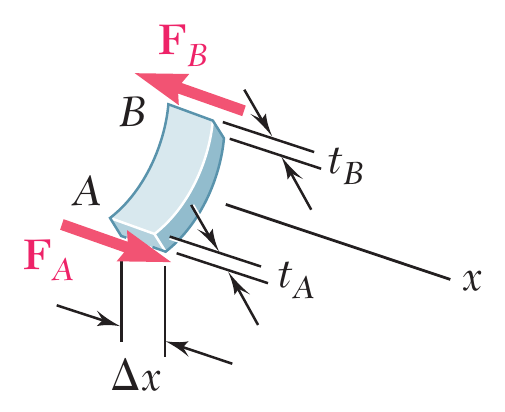
\includegraphics[width=\linewidth,height=1.4cm,keepaspectratio]{Chap_3/fig_3_49.png}\\[2pt]
      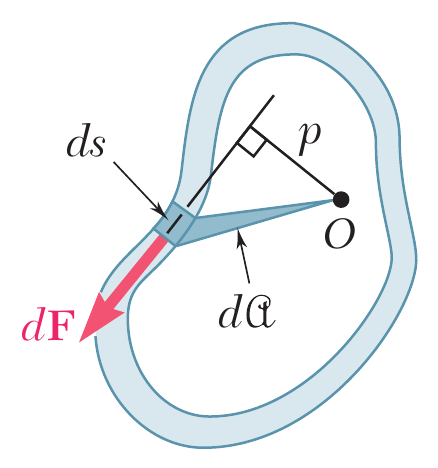
\includegraphics[width=\linewidth,height=1.4cm,keepaspectratio]{Chap_3/fig_3_53.png}\\[2pt]
      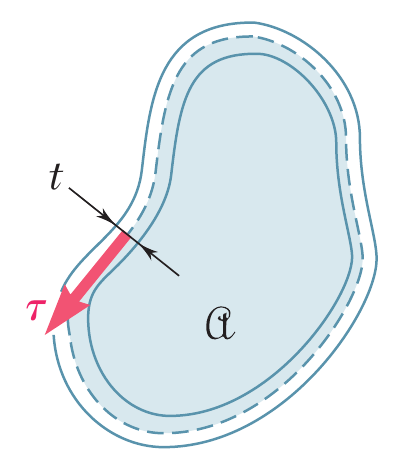
\includegraphics[width=\linewidth,height=1.4cm,keepaspectratio]{Chap_3/fig_3_54.png}
  \end{columns}
\end{frame}
% ===========
\section{Ví dụ 3.10}
\begin{frame}[t]{Ví dụ 3.10}
  \begin{columns}[T]
    \column{0.40\textwidth}
      \centering
      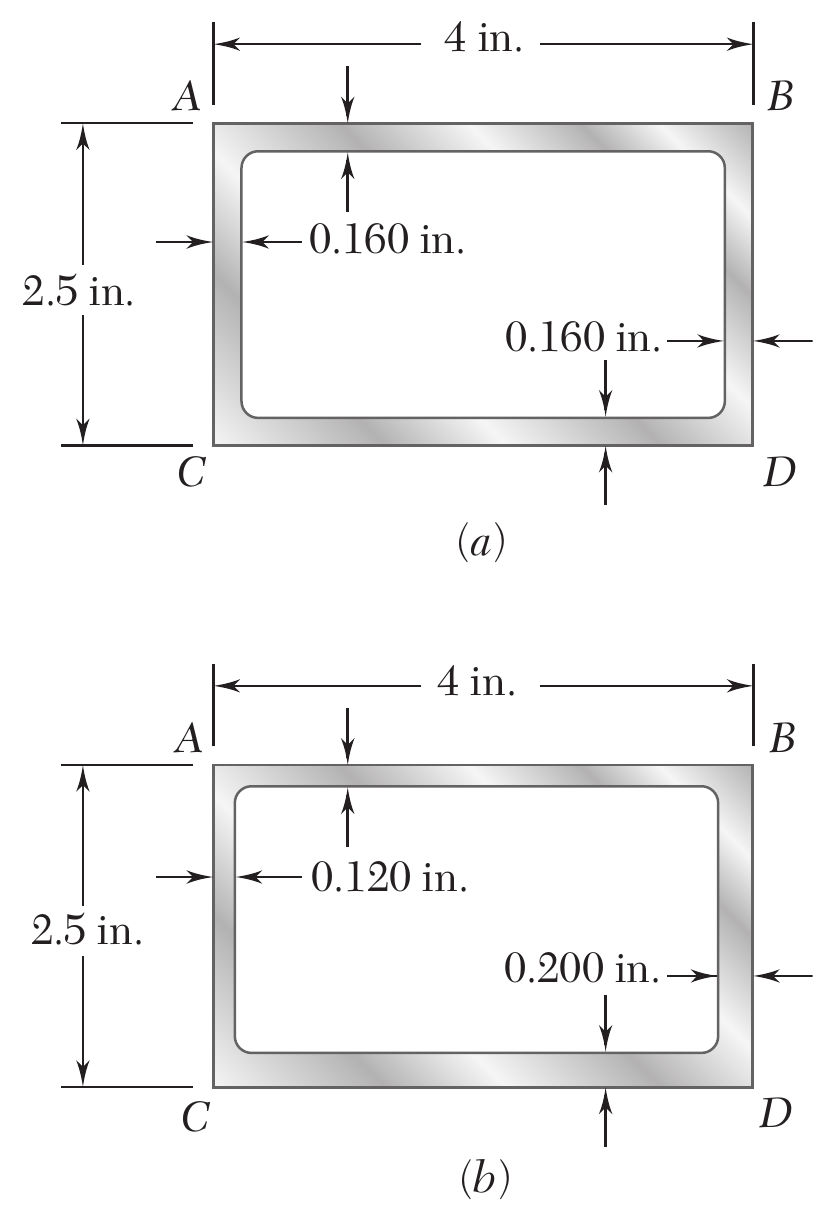
\includegraphics[width=\linewidth,height=5.5cm,keepaspectratio]{Chap_3/fig_3_55_a.png}
    \column{0.58\textwidth}
      \small
      Ống nhôm đùn có mặt cắt hình chữ nhật chịu mô men xoắn
      $2{,}7\,\mathrm{kN\cdot m}$. Xác định ứng suất tiếp trên mỗi thành
      trong bốn thành ống với (a) chiều dày thành đều bằng 4 mm và (b)
      chiều dày thành bằng 3 mm trên $AB$ và $AC$, 5 mm trên $CD$ và $BD$.

      \vspace{0.8em}
      \textbf{LỜI GIẢI:}
      \begin{itemize}
        \setlength{\itemsep}{0.5em}
        \item Xác định dòng lực cắt qua các thành ống.
        \item Tìm ứng suất tiếp tương ứng với từng chiều dày thành.
      \end{itemize}
  \end{columns}
\end{frame}
% ===========
\begin{frame}[t]{Ví dụ 3.10 (tiếp)}
  \begin{columns}[T]
    \column{0.45\textwidth}
      \small
      \textbf{LỜI GIẢI:}
      \begin{itemize}
        \item Xác định dòng lực cắt qua các thành ống:
      \end{itemize}
      \[
        \mathcal{A} = (96\,\mathrm{mm})(56\,\mathrm{mm}) = 5376\,\mathrm{mm}^2
      \]
      \[
        q = \frac{T}{2\mathcal{A}}
          = \frac{2700\,\mathrm{N\cdot m}}{2(5376\times10^{-6}\,\mathrm{m}^2)}
      \]
      \[
        q = 251{,}1\times10^{3}\,\mathrm{N/m}
      \]
      \centering
      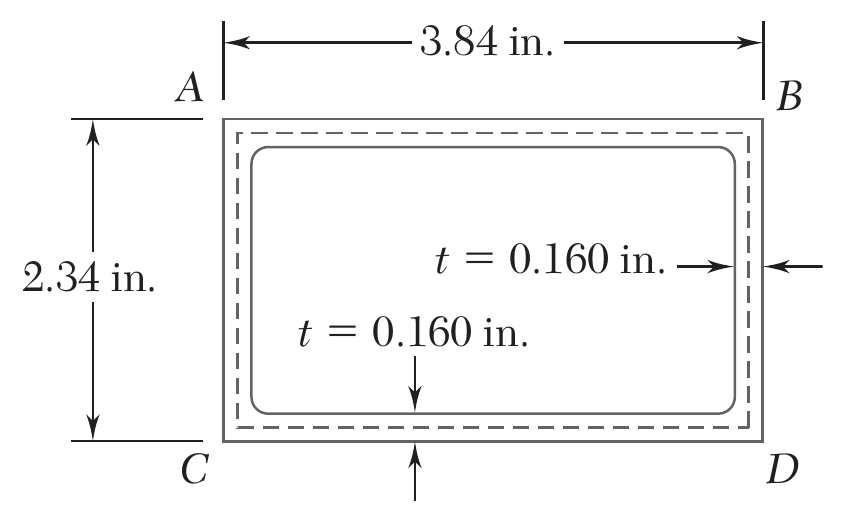
\includegraphics[width=0.8\linewidth,height=2.8cm,keepaspectratio]{Chap_3/fig_3_55_b.png}
    \column{0.53\textwidth}
      \small
      \begin{itemize}
        \item Tìm ứng suất tiếp tương ứng với từng chiều dày thành.
      \end{itemize}
      Với chiều dày thành đều:
      \[
        \tau = \frac{q}{t} = \frac{251{,}1\times10^{3}}{0{,}004}
        \qquad \boxed{\tau = 62{,}8\,\mathrm{MPa}}
      \]
      Với chiều dày thành thay đổi:
      \[
        \tau_{AB} = \tau_{AC} = \frac{251{,}1\times10^{3}}{0{,}003}
        \qquad \boxed{83{,}7\,\mathrm{MPa}}
      \]
      \[
        \tau_{BD} = \tau_{CD} = \frac{251{,}1\times10^{3}}{0{,}005}
        \qquad \boxed{50{,}2\,\mathrm{MPa}}
      \]
  \end{columns}
\end{frame}

\end{document}
